\documentclass[]{article}
\usepackage{lmodern}
\usepackage{amssymb,amsmath}
\usepackage{ifxetex,ifluatex}
\usepackage{fixltx2e} % provides \textsubscript
\ifnum 0\ifxetex 1\fi\ifluatex 1\fi=0 % if pdftex
  \usepackage[T1]{fontenc}
  \usepackage[utf8]{inputenc}
\else % if luatex or xelatex
  \ifxetex
    \usepackage{mathspec}
  \else
    \usepackage{fontspec}
  \fi
  \defaultfontfeatures{Ligatures=TeX,Scale=MatchLowercase}
\fi
% use upquote if available, for straight quotes in verbatim environments
\IfFileExists{upquote.sty}{\usepackage{upquote}}{}
% use microtype if available
\IfFileExists{microtype.sty}{%
\usepackage{microtype}
\UseMicrotypeSet[protrusion]{basicmath} % disable protrusion for tt fonts
}{}
\usepackage[margin=1in]{geometry}
\usepackage{hyperref}
\hypersetup{unicode=true,
            pdftitle={Ciência de Dados para Todos (Data Science For All) - 2018.1 - Análise da Produção Científica e Acadêmica da Universidade de Brasília - Relatório Final da Disciplina - Departamento de Ciência da Computação da UnB},
            pdfauthor={Jorge H. C. Fernandes, Ricardo B. Sampaio, João Ribas de Moura e Jerônimo A. Filho},
            pdfborder={0 0 0},
            breaklinks=true}
\urlstyle{same}  % don't use monospace font for urls
\usepackage{color}
\usepackage{fancyvrb}
\newcommand{\VerbBar}{|}
\newcommand{\VERB}{\Verb[commandchars=\\\{\}]}
\DefineVerbatimEnvironment{Highlighting}{Verbatim}{commandchars=\\\{\}}
% Add ',fontsize=\small' for more characters per line
\usepackage{framed}
\definecolor{shadecolor}{RGB}{248,248,248}
\newenvironment{Shaded}{\begin{snugshade}}{\end{snugshade}}
\newcommand{\KeywordTok}[1]{\textcolor[rgb]{0.13,0.29,0.53}{\textbf{#1}}}
\newcommand{\DataTypeTok}[1]{\textcolor[rgb]{0.13,0.29,0.53}{#1}}
\newcommand{\DecValTok}[1]{\textcolor[rgb]{0.00,0.00,0.81}{#1}}
\newcommand{\BaseNTok}[1]{\textcolor[rgb]{0.00,0.00,0.81}{#1}}
\newcommand{\FloatTok}[1]{\textcolor[rgb]{0.00,0.00,0.81}{#1}}
\newcommand{\ConstantTok}[1]{\textcolor[rgb]{0.00,0.00,0.00}{#1}}
\newcommand{\CharTok}[1]{\textcolor[rgb]{0.31,0.60,0.02}{#1}}
\newcommand{\SpecialCharTok}[1]{\textcolor[rgb]{0.00,0.00,0.00}{#1}}
\newcommand{\StringTok}[1]{\textcolor[rgb]{0.31,0.60,0.02}{#1}}
\newcommand{\VerbatimStringTok}[1]{\textcolor[rgb]{0.31,0.60,0.02}{#1}}
\newcommand{\SpecialStringTok}[1]{\textcolor[rgb]{0.31,0.60,0.02}{#1}}
\newcommand{\ImportTok}[1]{#1}
\newcommand{\CommentTok}[1]{\textcolor[rgb]{0.56,0.35,0.01}{\textit{#1}}}
\newcommand{\DocumentationTok}[1]{\textcolor[rgb]{0.56,0.35,0.01}{\textbf{\textit{#1}}}}
\newcommand{\AnnotationTok}[1]{\textcolor[rgb]{0.56,0.35,0.01}{\textbf{\textit{#1}}}}
\newcommand{\CommentVarTok}[1]{\textcolor[rgb]{0.56,0.35,0.01}{\textbf{\textit{#1}}}}
\newcommand{\OtherTok}[1]{\textcolor[rgb]{0.56,0.35,0.01}{#1}}
\newcommand{\FunctionTok}[1]{\textcolor[rgb]{0.00,0.00,0.00}{#1}}
\newcommand{\VariableTok}[1]{\textcolor[rgb]{0.00,0.00,0.00}{#1}}
\newcommand{\ControlFlowTok}[1]{\textcolor[rgb]{0.13,0.29,0.53}{\textbf{#1}}}
\newcommand{\OperatorTok}[1]{\textcolor[rgb]{0.81,0.36,0.00}{\textbf{#1}}}
\newcommand{\BuiltInTok}[1]{#1}
\newcommand{\ExtensionTok}[1]{#1}
\newcommand{\PreprocessorTok}[1]{\textcolor[rgb]{0.56,0.35,0.01}{\textit{#1}}}
\newcommand{\AttributeTok}[1]{\textcolor[rgb]{0.77,0.63,0.00}{#1}}
\newcommand{\RegionMarkerTok}[1]{#1}
\newcommand{\InformationTok}[1]{\textcolor[rgb]{0.56,0.35,0.01}{\textbf{\textit{#1}}}}
\newcommand{\WarningTok}[1]{\textcolor[rgb]{0.56,0.35,0.01}{\textbf{\textit{#1}}}}
\newcommand{\AlertTok}[1]{\textcolor[rgb]{0.94,0.16,0.16}{#1}}
\newcommand{\ErrorTok}[1]{\textcolor[rgb]{0.64,0.00,0.00}{\textbf{#1}}}
\newcommand{\NormalTok}[1]{#1}
\usepackage{longtable,booktabs}
\usepackage{graphicx,grffile}
\makeatletter
\def\maxwidth{\ifdim\Gin@nat@width>\linewidth\linewidth\else\Gin@nat@width\fi}
\def\maxheight{\ifdim\Gin@nat@height>\textheight\textheight\else\Gin@nat@height\fi}
\makeatother
% Scale images if necessary, so that they will not overflow the page
% margins by default, and it is still possible to overwrite the defaults
% using explicit options in \includegraphics[width, height, ...]{}
\setkeys{Gin}{width=\maxwidth,height=\maxheight,keepaspectratio}
\IfFileExists{parskip.sty}{%
\usepackage{parskip}
}{% else
\setlength{\parindent}{0pt}
\setlength{\parskip}{6pt plus 2pt minus 1pt}
}
\setlength{\emergencystretch}{3em}  % prevent overfull lines
\providecommand{\tightlist}{%
  \setlength{\itemsep}{0pt}\setlength{\parskip}{0pt}}
\setcounter{secnumdepth}{0}
% Redefines (sub)paragraphs to behave more like sections
\ifx\paragraph\undefined\else
\let\oldparagraph\paragraph
\renewcommand{\paragraph}[1]{\oldparagraph{#1}\mbox{}}
\fi
\ifx\subparagraph\undefined\else
\let\oldsubparagraph\subparagraph
\renewcommand{\subparagraph}[1]{\oldsubparagraph{#1}\mbox{}}
\fi

%%% Use protect on footnotes to avoid problems with footnotes in titles
\let\rmarkdownfootnote\footnote%
\def\footnote{\protect\rmarkdownfootnote}

%%% Change title format to be more compact
\usepackage{titling}

% Create subtitle command for use in maketitle
\newcommand{\subtitle}[1]{
  \posttitle{
    \begin{center}\large#1\end{center}
    }
}

\setlength{\droptitle}{-2em}
  \title{Ciência de Dados para Todos (Data Science For All) - 2018.1 - Análise da
Produção Científica e Acadêmica da Universidade de Brasília - Relatório
Final da Disciplina - Departamento de Ciência da Computação da UnB}
  \pretitle{\vspace{\droptitle}\centering\huge}
  \posttitle{\par}
  \author{Jorge H. C. Fernandes, Ricardo B. Sampaio, João Ribas de Moura e
Jerônimo A. Filho}
  \preauthor{\centering\large\emph}
  \postauthor{\par}
  \predate{\centering\large\emph}
  \postdate{\par}
  \date{11/06/2018}


\begin{document}
\maketitle

\begin{verbatim}
## Warning: package 'readxl' was built under R version 3.4.4
\end{verbatim}

\begin{verbatim}
## Warning: package 'tidyr' was built under R version 3.4.4
\end{verbatim}

\begin{verbatim}
## Warning: package 'reshape2' was built under R version 3.4.4
\end{verbatim}

\begin{verbatim}
## 
## Attaching package: 'reshape2'
\end{verbatim}

\begin{verbatim}
## The following object is masked from 'package:tidyr':
## 
##     smiths
\end{verbatim}

\begin{verbatim}
## Warning: package 'tidyverse' was built under R version 3.4.4
\end{verbatim}

\begin{verbatim}
## Warning: package 'ggplot2' was built under R version 3.4.4
\end{verbatim}

\begin{verbatim}
## Warning: package 'tibble' was built under R version 3.4.4
\end{verbatim}

\begin{verbatim}
## Warning: package 'readr' was built under R version 3.4.4
\end{verbatim}

\begin{verbatim}
## Warning: package 'purrr' was built under R version 3.4.4
\end{verbatim}

\begin{verbatim}
## Warning: package 'forcats' was built under R version 3.4.4
\end{verbatim}

\section{Introdução}\label{introducao}

O presente relatório tem por objetivo descrever e analisar 3 programas
de pós-graduação da UNB, tendo como foco principal dois programas de
Pós-Graduação em Matemática da UnB e o programa de Ensino em Ciências.
Serão analisados o contexto dos programas de pós-graduação (PPG), para
que sejam expostas de maneira organizada as informações levantadas pelos
datasets disponibilizados pela plataforma do E-Lattes. Também serão
propostas relações com outras bases de dados da UNB como a base do
DGP(dados de grupos de pesquisa) e da base OASIS que contém informações
sobre as produções nacionais. A metodologia de análise a ser seguida é
uma aproximação ao CRISP-DM que visa unificar as formas de se realizar
mineração de dados, para que os procedimentos possam ser reproduzidos e
possuem algum nivel de confiabilizade com relação ao resultados obtidos.

\ldots{}

\section{Metodologia}\label{metodologia}

\subsection{Delimitações iniciais}\label{delimitacoes-iniciais}

Em aderência à estrutura do CRISP-DM, algumas delimitações de contexto
para o trabalho são apresentadas a seguir:

\subsubsection{Domínio de Aplicação do
projeto}\label{dominio-de-aplicacao-do-projeto}

O domínio de aplicação do projeto é o da produção científica e acadêmica
brasileira, mais específicamente a produção científica ou produção
acadêmica de um subgrupo de pesquisadores vinculados à Universidade de
Brasília. O domínio de aplicação do projeto deve ser declarado na
introdução ao relatório.

\subsubsection{Tipo de Problema
abordado}\label{tipo-de-problema-abordado}

O tipo de problema abordado é o da produção de análises descritivas,
quantitativas e de modelagem computacional ou estatística, que permitam
caracterizar como e porque ocorre a produção científica e acadêmica de
um grupo de pesquisadores. Essa caracterização visa subsidiar a tomada
de decisão por membros do Sistema Nacional de Pós-Graduação. O tipo de
problema abordado no projeto deve ser declarado na introdução ao
relatório.

\subsection{Modelo de Referência
CRISP-DM}\label{modelo-de-referencia-crisp-dm}

Miner (2012), aprofunda: ``(\ldots{}) In CRISP-DM, the complete life
cycle of a data mining project is represented with \textbf{six phases}:
business understanding (determining the purpose of the study), data
understanding (data exploration and understanding), data preparation,
modeling, evaluation, and deployment.(\ldots{}). {[}Miner, Gary.
Practical Text Mining and Statistical Analysis for Non-structure Text
Data Applications. Academic Press, 2012.{]}

\subsubsection{Por que usar o CRISP-DM?}\label{por-que-usar-o-crisp-dm}

Imagine uma analogia entre um projeto de datamining e a preparação de
uma receita de bolo para ser usada em uma fábrica. Para iniciar a
produção, com base numa receita de comprovada eficácia (metodológica e
científica), você tem que minerar os ingredientes (dados) em um grande
supermercado (\emph{dataset}). Com os ingredientes você precisa aplicar
um método (a forma de misturá-los), colocar os ingredientes numa
determinada ordem, mexer por um certo tempo, aquecer por tantos minutos
até o bolo ficar pronto e ser aprovado em um ou mais testes de
degustação.

Tendo por objetivo fazer com que essa receita (script de mineração de
dados) possa ser executada com sucesso diversas vezes, numa fábrica,
será que outro cozinheiro (cientista) que reproduzisse a receita
(método) chegaria ao mesmo resultado? Se a metodologia (receita) já foi
bastante testada, então é bem provável que o resultado será o mesmo e
seu produto (receita de bolo) será aceito para a produção
(\emph{deployment}) de análises para consumo futuro, com base em
fundamentos científicos.

\subsubsection{Organização hierárquica de atividades em
fases}\label{organizacao-hierarquica-de-atividades-em-fases}

Dentro de cada fase no CRISP-DM existe uma estrutura hierárquica de
atividades genéricas para serem realizadas. Cada uma dessas atividades
\textbf{genéricas} pode determinar a execução de atividades
\textbf{específicas}.

Voltando ao exemplo do bolo, a atividade '' 1. Entendimento do Bolo''
poderia conter uma atividade genérica chamada ``1.1. Determinar para que
o bolo servirá (simples café da manhã? bolo de aniversário? bolo de
casamento?)``. Dentro dessa atividade genérica poderia haver atividades
específicas como ``1.1.1.Entrevistar o contratante para obter detalhes
de onde o bolo será usado?``; ``1.1.2. Conversar com os convidados sob
alguma necessidade especial (sem lactose? sem glútem?)``, etc.

\subsubsection{Seis Fases do CRISP-DM}\label{seis-fases-do-crisp-dm}

Com base no apresentado, segue uma descrição um pouco mais detalhada das
seis fases de um projeto no CRISP-DM, interpretadas no contexto deste
relatório.

\paragraph{Entendimento do Negócio}\label{entendimento-do-negocio}

É o desenvolvimento dos objetivos e declaração das necessidades do
projeto sob a perspectiva do negócio, para transformar isso tudo em
definição de um problema de data mining. No caso desse relatório irá se
buscar encontrar dados referentes aos perfis, publicações e orientações
dos discentes dos programas de pós-graduação em matemática, . . . , .
Deve-se também definir um grupo de objetivos, um plano para a realização
do projeto e um critério de sucesso. Como objetivo para a parte de
datamining desse relatório tem-se conseguir dados referentes às
seguintes áreas:

\begin{itemize}
\tightlist
\item
  Áreas com resultados mais relevantes / expressivos;
\item
  Nível de Internacionalização;
\item
  Principais congressos e eventos da área no Brasil e no mundo;
\item
  Principais revistas e local de publicação de trabalhos no Brasil e no
  mundo;
\item
  Quantitativo de pessoas e programas dentro do universo;
\item
  Grupos de pesquisa associados ou que os professores / pesquisadores
  fazem parte.
\end{itemize}

Quanto ao plano para realização do projeto, será realizada as seguintes
etapas: * Tratamento dos dados para transformá-lo em um dataset; *
Análise dos dados para a criação de resultados relevantes; * Análise dos
resultados para encontrar os dados citados nos objetivos.

\paragraph{Entendimento dos Dados}\label{entendimento-dos-dados}

O segundo estágio do CRISP-DM requer que se tenha acesso ao dado listado
nos recursos do projeto. Essa fase requer a realização da descrição,
exploração, verificação da qualidade e relatório da qualidade dos dados.

Os dados analisados nesse relatório foram pegos a partir do arquivo
Matematica.profile.json que representa o dataset do programa de pós
graduação em Matemática (código: 53001010003P2) e conta com uma lista de
docentes e seus dados pessoais. Essa descrição e exploração foi feita
utilizando do comando View no rstudio. A qualidade dos dados se encontra
bastante satisfatória, com alguns problemas na padronização de alguns
dados como o endereço que em alguns casos apresenta diferentes nomes
para um mesmo curso como ``Matematica'' e ``Matemática''.

\paragraph{Preparação dos Dados}\label{preparacao-dos-dados}

Aqui os dados são ``filtrados'' retirando-se partes que não interessam e
selecionando-se os ``campos'' necessários para o trabalho de mineração.
São 5 as atividades genéricas nesta fase de preparação dos dados:

\begin{itemize}
\tightlist
\item
  Seleção dos dados. Envolve identificar quais dados, da nossa
  ``montanha de dados'', serão realmente utilizados. Quais variáveis dos
  dados brutos serão convertidas para o dataset? Não é raro cometer o
  erro de selecionar dados para um modelo preditivo com base em uma
  falsa ideia de que aqueles dados contém a resposta para o modelo que
  se quer construir. Surge o cuidado de se separar o sinal do ruído
  (Silver, Nate. The Signal and the Noise: Why so many predictions fail
  --- but some don't. USA: The Penguin Press HC, 2012.).
\item
  Limpeza dos dados.
\item
  Construção dos dados. Envolve a criação de novas variáveis a partir de
  outras presentes nos \texttt{datasets.}
\item
  Integração dos dados. Envolve a união (merge) de diferentes tabelas
  para criar um único \texttt{dataset} para ser utilizado no R, por
  exemplo.
\item
  Formatação dos dados. Envolve a realização de pequenas alterações na
  estrutura dos dados, como a ordem das variáveis, para permitir a
  execução de determinado método de data mining.
\end{itemize}

\paragraph{Modelagem}\label{modelagem}

No CRISP-DM este estágio envolve a construção e avaliação do modelo,
podendo ser realizada em quatro atividades genéricas: * Seleção das
técnicas de modelagem; * Realização de testes de modelagem, onde
diferentes modelos são previamente testados e avaliados. Pode-se dividir
o dataset criado na etapa anterior para se ter uma base de treino na
construção de modelos, e outra pequena parte para validar e avaliar a
eficiência de cada modelo criado até se chegar ao mais ``eficiente''. *
Construção do modelo definitivo, com base na melhor experiência do passo
anterior. * Avaliação do modelo.

\paragraph{Avaliação}\label{avaliacao}

Aqui os resultados não são apenas avaliados, mas se verifica se existem
questões relacionadas à organização que não foram suficientemente
abordadas. Deve-se refletir se o uso arepetido do modelo criado pode
trazer algum ``efeito colateral'' para a organização.

Nesta fase, pode-se trabalhar com 3 atividades genéricas: * Avaliação
dos resultados; * Revisão do processo, por meio da qual verifica-se se o
modelo foi construído adequadamente. As variáveis (passadas) para
construir o modelo estarão disponíveis no futuro? * Determinação dos
etapas seguintes. Pode ser necessário decidir-se por finalizar o
projeto, passar à etapa de desenvolvimento, ou rever algumas fases
anteriores para a melhoria do projeto.

\paragraph{\texorpdfstring{Implantação
(\texttt{deployment})}{Implantação (deployment)}}\label{implantacao-deployment}

Foi realizado o planejamento de implantação dos produtos desenvolvidos
(scripts, no caso do executado nesta disciplina) para o ambiente
operacional, para seu uso repetitivo, envolvendo atividades de
monitoramento e manutenção do sistema (script) desenvolvido. A fase de
implantação concluir com a produção e apresentação do relatório final
com os resultados do projeto.

São atividades genéricas na fase de \textbf{implantação}: * Planejamento
da transição dos produtos; * Planejamento do monitoramento dos produtos
em utilização no ambiente operacional; * Planejamento de manuteção a ser
eventualmente efetuada no produto (scripts); * Produção do relatório
final; * Apresentação do relatório final; * Revisão sobre a execução do
projeto, com registro de lições aprendidas.

No contexto do projeto realizado no âmbito desta disciplina, a
responsabilidade por execução de todas essas atividades é dos alunos,
com exceção da apresentação do relatório final, que não será realizada.

\section{CRISP-DM Fase 1 - Entendimento do
Negócio}\label{crisp-dm-fase-1---entendimento-do-negocio}

\subsection{O que é o Sistema Nacional de Pós-Graduação?
(Contextualização)}\label{o-que-e-o-sistema-nacional-de-pos-graduacao-contextualizacao}

A produção do conhecimento científico, no Brasil, é predominantemente
efetuada por meio do Sistema Nacional de Pós-Graduação - SNPG, e mais
fortemente relacionada com a formação de doutores nesse sistema (Pátaro
e Mezzomo, 2013), por meio de cursos de pós-graduação \emph{strictu
sensu}.

Fernandes e Sampaio (2017) já indicaram que a ciência é reconhecidamente
um elemento essencial para o desenvolvimento social e econômico de
qualquer nação. Assim sendo, faz-se mister aprimorar o SNPG como forma
de promoção desse crescimento, visando maximizar o retorno decorrente do
emprego dos recursos nele aplicados. A promoção do crescimento do SNPG
se dá predominantemente por meio de avaliações regulares de seus
programas de pós-graduação, sob responsabilidade da CAPES, que realiza a
cada quatro anos um complexo (Leite, 2018, p.~13) e custoso processo de
coleta de dados, análise e deliberação sobre as pós-graduações
\emph{strictu sensu}, em coerência com o estabelecido no Plano Nacional
de Pós-Graduação (PNPG) 2012-2020 (CAPES, 2010) e nos diversos
documentos que definem os critérios de organização da pós-graduação em
cada área do conhecimento (CAPES, 2018). Leite (2018) faz uma
apresentação geral de como se organizam e são avaliadas as
pós-graduações no Brasil.

O Plano Nacional de Pós-Graduação (PNPG), por outro lado, define
diretrizes estratégicas para desenvolvimento da pós-graduação
brasileira, que deve abordar prioritariamente grandes temas de interesse
nacional, tais como a redução das assimetrias de desenvolvimento entre
as regiões do Brasil, a formação de professores para a educação básica,
a formação de recursos humanos para as empresas, a resposta aos grandes
desafios brasileiros sobre Água, Energia, Transporte, Controle de
Fronteiras, Agronegócio, Amazônia, Amazônia Azul (Mar), Saúde, Defesa,
Programa Espacial, além de Justiça, Segurança Pública, Criminologia e
Desequilíbrio Regional. O PNPG também traça as diretrizes para
financiamento da pós-graduação e sua internacionalização, apresentando
conclusões e recomendações.

As avaliações do SNPG, ao atribuirem mensurações de desempenho às
diversas pós-graduações que dele fazem parte, geram incentivos e
penalidades aos programas, tendo em vista a limitada disponibilidade de
recursos para investimento em bolsas, taxas de bancada etc. Embora o
sistema seja altamente sofisticado ele é também altamente criticado
(Azevedo et al., 2016), sobretudo porque há percalços na busca por um
equilíbrio entre as diferentes concepções de finalidade da ciência. Se
de um lado a promoção do conhecimento gerado predominantemente nas ditas
ciências \emph{hard} constribui para criar fluxos econômicos mais
intensos, isso não significa que essa promoção possa ocorrer em
detrimento da menor promoção na geração de conhecimento sobre problemas
sociais, predominantemente gerado nas ditas ciências \emph{soft},
especialmente das áreas de humanidades, sob pena de ampliação de
desigualdades (Azevedo et al., 2016).

Não há solução simples, mas postula-se, nesta disciplina, que uma maior
agilidade na avaliação e a utilização de critérios mais objetivos,
poderá facilitar a melhoria do sistema.

\subsubsection{Os Colégios, Grandes Áreas e Áreas da Pós-Graduação
Brasileira}\label{os-colegios-grandes-areas-e-areas-da-pos-graduacao-brasileira}

A partir de 2018, as diversas áreas da pós-graduação brasileira foram
organizadas na forma de colégios, grandes áreas e áreas, conforme
apresentam as tabelas a seguir.

\paragraph{Colégio de Ciências da
vida}\label{colegio-de-ciencias-da-vida}

\begin{longtable}[]{@{}lll@{}}
\toprule
CIÊNCIAS AGRÁRIAS & CIÊNCIAS BIOLÓGICAS & CIÊNCIAS DA
SAÚDE\tabularnewline
\midrule
\endhead
Ciência de Alimentos & Biodiversidade & Educação Física\tabularnewline
Ciências Agrárias I & Ciências Biológicas I & Enfermagem\tabularnewline
Medicina Veterinária & Ciências Biológicas II & Farmácia\tabularnewline
Zootecnia / Recursos Pesqueiros & Ciências Biológicas III & Medicina
I\tabularnewline
- & - & Medicina II\tabularnewline
- & - & Medicina III\tabularnewline
- & - & Nutrição\tabularnewline
- & - & Odontologia\tabularnewline
- & - & Saúde Coletiva\tabularnewline
\bottomrule
\end{longtable}

\paragraph{Colégio de Ciências Exatas, Tecnológicas e
Multidisciplinar}\label{colegio-de-ciencias-exatas-tecnologicas-e-multidisciplinar}

\begin{longtable}[]{@{}lll@{}}
\toprule
CIÊNCIAS EXATAS E DA TERRA & ENGENHARIAS &
MULTIDISCIPLINAR\tabularnewline
\midrule
\endhead
Astronomia / Física & Engenharias I & Biotecnologia\tabularnewline
Ciência da Computação & Engenharias II & Ciências
Ambientais\tabularnewline
Geociências & Engenharias III & Ensino\tabularnewline
Matemática / Probabilidade e Estatística & Engenharias IV &
Interdisciplinar\tabularnewline
Química & - & Materiais\tabularnewline
\bottomrule
\end{longtable}

\paragraph{Colégio de Humanidades}\label{colegio-de-humanidades}

\begin{longtable}[]{@{}lll@{}}
\toprule
CIÊNCIAS HUMANAS & CIÊNCIAS SOCIAIS APLICADAS & LINGUÍSTICA, LETRAS E
ARTES\tabularnewline
\midrule
\endhead
Antropol/Arqueol & Admin.Púb./Empr.,C.Contáb. e Tur. &
Artes\tabularnewline
Ciência Pol. e Rel. Int. & Arquit., Urban. e Design & Linguística e
Literatura\tabularnewline
Ciências da Religião e Teol. & Comunicação e Informação &
-\tabularnewline
Educação & Direito & -\tabularnewline
Filosofia & Economia & -\tabularnewline
Geografia & Planej. Urbano e Reg. / Demografia & -\tabularnewline
História & Serviço Social & -\tabularnewline
Psicologia & - & -\tabularnewline
Sociologia & - & -\tabularnewline
\bottomrule
\end{longtable}

Cada um desses colégios, grandes áreas e áreas de conhecimento possuem
dinâmicas próprias, e, portanto, não há um modelo universal que se
aplique a todas. Existem aspectos comuns, mas também grandes
peculiaridades, descritas parcialmente nos correspondentes documentos de
área disponíveis em CAPES (2018).

\subsection{A UnB dentro do Sistema Nacional de Pós-Graduação
(Contextualização)}\label{a-unb-dentro-do-sistema-nacional-de-pos-graduacao-contextualizacao}

\subsubsection{O que é a UnB?}\label{o-que-e-a-unb}

A Universidade de Brasília é uma instituição de ensino superior composta
por cinco campus em Brasília e cidades satélites que oferecem formação
da graduação à pós-graduação. Do ponto de vista de sua produção
científica a UnB ocupa atualmente a posição número 737 no ranking
mundial de melhores universidades do mundo de acordo com o Center for
World University Rankings (CWUR), que leva em consideração
principalmente premiações, artigos, número de citações, pesquisas e
publicações.

Em relação às demais universidades do Brasil, segundo o Ranking de
Universidades Folha (2017) que classifica as melhores universidades do
país, entre as 296 instituições públicas de nível superior a UnB se
encontra na posição número 20 sendo a 11ª em número de teses publicadas,
a 10ª e número de publicações em revistas nacionais e a 20ª em núméro de
publicações por docente.

\subsubsection{Descrição das pós-graduações da
UnB}\label{descricao-das-pos-graduacoes-da-unb}

Neste trabalho o foco foi em três programas de pós-graduação da UNB.
Entre eles dois programas do departamento de matemática e outro do
programa de ensino em ciências. Nós próximos tópicos serão detalhados os
contextos de cada PPG sendo trabalhado.

\paragraph{Programa de Pós-graduação de ensino em
ciências}\label{programa-de-pos-graduacao-de-ensino-em-ciencias}

O programa de pós-graduação em ensino de ciências, tem como objetivo
qualificar os professores de nível básico em matérias relativas a
ciências e afins. O foco é dado no desenvolvimento de conteúdos de
ciências, o que envolve aspectos teóricos, metodológicos e
epistemológicos relativo ao ensino de ciências além do desenvolvimento e
aprendizado de novas tecnologias que permitam a evolução do ensino.

O programa engloba professores com as mais diversas áreas de atuação e
de diferentes cantos da universidade. Podemos citar como áreas a física,
bioquímica, ecologia, história, química, genética, medicina, psicologia
entre outras, com destaques para a participação do Instituto de Física,
Química e Ciências Biológicas. Os programas englobam três linhas de
pesquisa sendo elas: Ensino-Aprendizagem em Ciências da Natureza em seus
mutilplos aspectos; Formação de Professores de Ciências da Natureza e
Educação Científica e Cidadania.

A implementação do Programa de Pós-Graduação em Ensino de Ciências na
UnB, se deu inicialmente em 2007 e desde 2010, tem sido ampliado seu
quadro de docentes por meio do credenciamento de novos orientadores,
principalmente a partir da aproximação com o curso de Licenciatura em
Ciências Naturais da Faculdade UnB Planaltina.

O programa é composto por 19 professores que já realizaram cerca de 709
orientações ao longo dos anos de 2010 a 2017 com cerca de 174
dissertações de mestrado concluidas até o momento. Podemos observar
abaixo as distribuições de cada orientação realizada ao longo dos anos.
É possível observar um grande aumento na quantidade(relativa) de
orientações realizadas de mestrado, o que pode ser explicado pelo
aumento do número de novos orientadores credenciados ao PPG.

\includegraphics{Relatório_4_files/figure-latex/plot1-1.pdf}

Abaixo teremos as quantidades absolutas totais de orientações realizadas
ao longo dos anos de 2010 a 2017 apenas para complementar a distribuição
acima apresentada:

\includegraphics{Relatório_4_files/figure-latex/plot2-1.pdf}

Em média os orientadores possuem nível de senioridade 7, tendo 5 como
mínimo e 9 como máximo, o que indica que no geral os professores possuem
bastante experiência no meio acadêmico, e pode ser relevante para
explicar a quantidade de orientações realizadas pelo programa e também o
número de publicações realizadas. No total os orientadores participam de
29 grupos de pesquisa e são em sua totalidade nascidos no brasil com uma
idade média de 58 anos de idade. Entre os grupos aos quais os
orientadores participam podemos citar os de Educação Científica e
Cidadania, Ensino de Ciências e Mediação Pedagógica, Aprendizagem e
mediação pedagógica, Ecologia e Comportamento e o grupo de Ensino de
Química.

Atualmente estão sendo realizadas 74 orientações que incluem,
mestrandos, doutorandos e PHDs. Deste conjunto existem alunos que vieram
de diversas instituições, dentre elas Universidade Federal de Mato
Grosso, Universidade Federal de Pernambuco, Universidade Federal de
Sergipe e Centro Universitário Norte do Espírito Santo, porém nenhum
estudante proveniente de instituições internacionais.

\paragraph{Programas de Pós-graduação da
Matemática}\label{programas-de-pos-graduacao-da-matematica}

Aqui será feita uma contextualização das áreas de pesquisa relacionadas
ao programa de Pós-Graduação em Matemática da UnB, dos anos 2010 à 2017.
Para tal está sendo apresentado dados de produção científica dos
docentes do programa, retirados do currículo Lattes dos professores e do
repositório \texttt{OASIS} do \texttt{IBICT} (Instituto Brasileiro de
Informação em Ciência e Tecnologia).

O coordenador do PPG é o Carlos Alberto Pereira dos Santos e as subáreas
de concentração são: \textbf{Álgebra, Análise, Geometria e Matemática
Aplicada}. Mais informações do programa podem ser acessadas pelo site
\href{https://sucupira.capes.gov.br/sucupira/public/consultas/coleta/programa/viewPrograma.jsf?popup=true\&cd_programa=53001010003P2}{sucupira}.

O programa de Pós-Graduação em Matemática da UnB, iniciado em 1962,
oferece Mestrado e Doutorado em Matemática nas subáreas de Álgebra,
Análise, Geometria e Matemática Aplicada (Probabilidade,
Física-Matemática e Computação). O corpo docente mantém um programa
ativo de pesquisa, participa regular e ativamente de forma destacada em
reuniões científicas e em corpos editoriais de revistas científicas,
além de manter intercâmbio científico com diversas instituições do país
e do exterior.

Há também um programa de mestrado profissional \texttt{PROFMAT}, que é
um programa de pós-graduação stricto sensu em Matemática, reconhecido
pelo Ministério da Educação e conduzindo ao título de Mestre. Tem como
objetivo proporcionar formação matemática aprofundada relevante ao
exercício da docência no Ensino Básico, visando dar ao egresso a
qualificação certificada para o exercício da profissão de professor de
Matemática.

O \texttt{PROFMAT} é um curso semipresencial ministrado por Instituições
de Ensino Superior associadas em uma Rede Nacional, no âmbito do
\textbf{Sistema Universidade Aberta do Brasil} (UAB). É coordenado pela
Comissão Acadêmica Nacional, que opera sob a égide da Diretoria da
\textbf{Sociedade Brasileira de Matemática} (SBM).

As Instituições de Ensino Superior que integram a Rede Nacional do
\texttt{PROFMAT} são denominadas Instituições Associadas e são
responsáveis, por intermédio das respectivas Coordenações Acadêmicas
Institucionais, por toda a gestão local do \texttt{PROFMAT}, descritas
no Regimento. Informações completas sobre este mestrado podem ser
encontradas na página do
\href{http://www.profmat-sbm.org.br}{\texttt{PROFMAT}}. Na Universidade
de Brasília este curso é ofertado no âmbito do Instituto de Ciências
Exatas, Departamento de Matemática.

O Departamento de Matemática da UnB obteve nota 7 na última avaliação
trienal da Capes. Essa avaliação de excelência é o resultado de um
longo, árduo e contínuo trabalho iniciado em 1962 por
professores/colaboradores corajosos e idealistas que acreditaram em
tornar o sonho do Departamento de Matemática da Universidade de Brasília
uma realidade. Desde então, esse ideal vem sendo fortalecido com a
chegada de novos professores/colaboradores que conduziram este programa
ao reconhecimento da sua excelência.

\section{CRISP-DM Fase 2 - Entendimento dos
Dados}\label{crisp-dm-fase-2---entendimento-dos-dados}

\subsection{CRISP-DM Fase.Atividade 2.1 - Coleta inicial dos
dados}\label{crisp-dm-fase.atividade-2.1---coleta-inicial-dos-dados}

Todos os arquivos com dados iniciais a seguir apresentados foram
fornecidos pelos professores responsáveis pela disciplina. Os dados
foram gerados no mês de maio de 2018, e compilam informações entre os
anos de 2010 e 2017. Os arquivos estão no formato JSON, e seus atributos
iniciais e conteúdos são apresentados a seguir.

A metodologia utilizada tenta seguir o que é proposto pelo modelo
CRISP-DM. Inicialmente o contexto do programa de pós-graduação foi
explorado, buscando o máximo possível de informações sobre o PPG
incluindo seu funcionamento e suas áreas de pesquisa. Os dados foram
buscados e explorados a partir do website do programa com o intuito de
compreender melhor o contexto que será trabalhado.. Os dados utilizados
para pesquisa foram tirados do dataset de publicações, orientações e
perfis da Matemática do portal do programa e do
\href{http://unb.elattes.com.br/user/login}{elattes}.

Uma vez compreendido do que se trata o programa os dados dispostos pelo
E-Lattes foram explorados para um reconhecimento inicial. Pode-se notar
que os dados vieram em formato JSON, englobando os universos de
publicações, orientações, perfis e áreas de pesquisa dos orientadores do
departamento, além dos dados referentes as bases do DGP e OASIS. Após
importação devida os dados passaram por uma exploração inicial para
entender sua formatação e se alguma modificação seria necessária para
trabalhar com as ferramentas disponíveis framework da linguagem R.

Os dados constituem informações sobre os orientadores do departamento o
que inclui, senioridade, produções, endereço profissional, produção
bibliográfica e orientações que os mesmos realizaram. Também podemos
identificar informações sobre as orientações realizadas pelo
departamento que incluem informações sobre o aluno sendo orientado, como
curso, instituição, nome dos orientadores, título da orientação, ano e
qual estado se encontra a orientação, em andamento ou concluída. Por
último temos os dados de publicações que englobam 6 tipos de publicações
que serão detalhadas nos resultados obtidos.

Em seguida foi identificado que alguns dados não estavam totalmente
preparados para a realização de buscas, uma vez que é necessária a
formatação em tabelas (e não em listas) para a realização de filtragens
e joins de maneira clara prática. Portanto os arquivos de publicações e
perfis foram modificados para que fossem removidas algumas listas
internas a estruturam que dificultavam sua utilização. Por exemplo, no
arquivo de publicações, temos uma grande lista com 7 outras listas como
elementos: periódico, livro, capítulo de livro, texto em jornais,
evento, artigo aceito e demais tipos de produação bibliográfica.

Tendo os dados filtrados e organizados foram efetuadas consultas básicas
com o intuito de ter uma visualização mais clara dos conjuntos de dados.
As bibliotecas utilizadas para filtragem e visualização foram a
\texttt{dplyr}, que permitem consultas semelhantes a consultas de bancos
de dados, com dados organizadas em tabelas (em R conhecidas como
dataframes), e a biblioteca \texttt{ggplot2} que possibilita a fácil
criação de gráficos a parir de dataframes.

Após a realização das consultas foram geradas algumas conclusões que
foram cruzadas com os dados iniciais obtidos a partir da avaliação do
contexto do programa, apesar de o trabalho ter caráter expositivo foi
gerado um modelo para tentar explicar algumas situações identificadas ao
longo da pesquisa do PPG. O procedimento aqui demonstrado foi repetido
até que fossem obtidos resultados satisfatórios assim como descreve o
modelo CRISP-DM.

\subsubsection{Perfil profissional dos docentes vinculados às
pós-graduações}\label{perfil-profissional-dos-docentes-vinculados-as-pos-graduacoes}

\begin{Shaded}
\begin{Highlighting}[]
\NormalTok{json.perfil <-}\StringTok{ "Matematica.profile.json"}
\KeywordTok{file.info}\NormalTok{(json.perfil)}
\end{Highlighting}
\end{Shaded}

\begin{verbatim}
##                           size isdir mode               mtime
## Matematica.profile.json 654736 FALSE  666 2018-07-07 17:52:28
##                                       ctime               atime exe
## Matematica.profile.json 2018-07-07 17:52:28 2018-07-07 17:52:28  no
\end{verbatim}

O arquivo Matematica.profile.json apresenta dados sobre o perfil de
todos os docentes vinculados a programas de pós-graduação da UnB, entre
2010 e 2017. Esse arquivo foi fornecido pelos docentes responsáveis pela
disciplina.

\subsubsection{Orientações de mestrado e doutorado realizadas pelos
docentes vinculados às
pós-graduações}\label{orientacoes-de-mestrado-e-doutorado-realizadas-pelos-docentes-vinculados-as-pos-graduacoes}

\begin{Shaded}
\begin{Highlighting}[]
\NormalTok{json.advise <-}\StringTok{ "Matematica.advise.json"}
\KeywordTok{file.info}\NormalTok{(json.advise)}
\end{Highlighting}
\end{Shaded}

\begin{verbatim}
##                          size isdir mode               mtime
## Matematica.advise.json 235679 FALSE  666 2018-07-07 17:52:28
##                                      ctime               atime exe
## Matematica.advise.json 2018-07-07 17:52:28 2018-07-07 17:52:28  no
\end{verbatim}

O arquivo Matematica.advise.json apresenta dados sobre o orientações de
mestrado e doutorado feitas por todos os docentes vinculados a programas
de pós-graduação da UnB, entre 2010 e 2017. Esse arquivo foi fornecido
pelos docentes responsáveis pela disciplina.

\subsubsection{Produção bibliográfica gerada pelos docentes vinculados
às
pós-graduações}\label{producao-bibliografica-gerada-pelos-docentes-vinculados-as-pos-graduacoes}

\begin{Shaded}
\begin{Highlighting}[]
\NormalTok{json.producao.bibliografica <-}\StringTok{ "Matematica.publication.json"}
\KeywordTok{file.info}\NormalTok{(json.producao.bibliografica) }
\end{Highlighting}
\end{Shaded}

\begin{verbatim}
##                               size isdir mode               mtime
## Matematica.publication.json 313273 FALSE  666 2018-07-07 17:52:28
##                                           ctime               atime exe
## Matematica.publication.json 2018-07-07 17:52:28 2018-07-07 17:52:28  no
\end{verbatim}

O arquivo Matematica.publication.json apresenta dados sobre a produção
bibliográfica gerada por todos os docentes vinculados a programas de
pós-graduação da UnB, entre 2010 e 2017.

\subsubsection{Agrupamento dos docentes conforme áreas de
atuação}\label{agrupamento-dos-docentes-conforme-areas-de-atuacao}

\begin{Shaded}
\begin{Highlighting}[]
\NormalTok{json.researchers_by_area <-}\StringTok{ "Matematica.researchers_by_area.json"} 
\KeywordTok{file.info}\NormalTok{(json.researchers_by_area)}
\end{Highlighting}
\end{Shaded}

\begin{verbatim}
##                                     size isdir mode               mtime
## Matematica.researchers_by_area.json 1161 FALSE  666 2018-07-07 17:52:28
##                                                   ctime
## Matematica.researchers_by_area.json 2018-07-07 17:52:28
##                                                   atime exe
## Matematica.researchers_by_area.json 2018-07-07 17:52:28  no
\end{verbatim}

O arquivo Matematica.researchers\_by\_area.json apresenta as vinculações
de todos os docentes que declararam atuar em cada uma das áreas de
pós-graduação do Sistema Nacional de Pós-Graduação da CAPES, conforme
apresenta-se registrada essa informação no currículo Lattes de cada um,
em data recente.

\begin{Shaded}
\begin{Highlighting}[]
\KeywordTok{file.info}\NormalTok{(}\StringTok{'Matematica.graph.json'}\NormalTok{)}
\end{Highlighting}
\end{Shaded}

\begin{verbatim}
##                       size isdir mode               mtime
## Matematica.graph.json 6179 FALSE  666 2018-07-07 17:52:28
##                                     ctime               atime exe
## Matematica.graph.json 2018-07-07 17:52:28 2018-07-07 17:52:28  no
\end{verbatim}

\subsection{CRISP-DM Fase.Atividade 2.2 - Descrição dos
Dados}\label{crisp-dm-fase.atividade-2.2---descricao-dos-dados}

Para ler e manipular inicialmente esses dados, serão usadas
primordialmente as bibliotecas seguintes

\begin{Shaded}
\begin{Highlighting}[]
\KeywordTok{library}\NormalTok{(jsonlite)}
\KeywordTok{library}\NormalTok{(listviewer)}
\end{Highlighting}
\end{Shaded}

\begin{verbatim}
## Warning: package 'listviewer' was built under R version 3.4.4
\end{verbatim}

\begin{Shaded}
\begin{Highlighting}[]
\KeywordTok{library}\NormalTok{(readxl)}
\KeywordTok{library}\NormalTok{(readr)}
\CommentTok{#library(readtext)}
\KeywordTok{library}\NormalTok{(ggplot2)}
\KeywordTok{suppressMessages}\NormalTok{(}\KeywordTok{library}\NormalTok{(}\StringTok{"tidyverse"}\NormalTok{))}
\end{Highlighting}
\end{Shaded}

Como já informado, a descrição dos dados verifica se os dados sendo
acessados terão potencial para responder às questões de \emph{data
mining}. Além disso, deve-se avaliar qual o volume de dados, a estrutura
dos dados (tipos), codificações usadas, etc. Neste projeto, a descrição
dos dados é responsabilidade parcial dos alunos, tendo em vista que esta
seção já oferece uma descrição inicial simplificada. O relatório final
deve conter descrições significativas e aprofundadas dos dados.

\subsubsection{Descrição dos dados do
perfil}\label{descricao-dos-dados-do-perfil}

O arquivo unb.perfis.json, que contém dados que caracterizam o perfil
profissional de todos os docentes do grupo sob análise, podem ser lido
por meio do comando seguinte.

\begin{Shaded}
\begin{Highlighting}[]
\NormalTok{unb.prof <-}\StringTok{ }\KeywordTok{fromJSON}\NormalTok{(}\StringTok{"Matematica.profile.json"}\NormalTok{)}
\end{Highlighting}
\end{Shaded}

A quantidade de docentes sob análise é apresentada a seguir.

\begin{Shaded}
\begin{Highlighting}[]
\KeywordTok{length}\NormalTok{(unb.prof)}
\end{Highlighting}
\end{Shaded}

\begin{verbatim}
## [1] 44
\end{verbatim}

Para gerar uma apresentação inicial dos dados que estão contido nos
dados de perfil dos docentes, pode-se usar a função glimpse, da
biblioteca dplyr, como ilustra o código seguinte, que apresenta os
atributos típicos que podem ser obtidos relativamente a um pesquisador
específico, o mais antigo docente ainda em exercício na UnB a ter criado
seu registro na plataforma Lattes.

\begin{Shaded}
\begin{Highlighting}[]
\KeywordTok{library}\NormalTok{(dplyr) }
\KeywordTok{glimpse}\NormalTok{(unb.prof[[}\DecValTok{1}\NormalTok{]], }\DataTypeTok{width =} \DecValTok{30}\NormalTok{)}
\end{Highlighting}
\end{Shaded}

\begin{verbatim}
## List of 7
##  $ nome                  : chr "Norai Romeu Rocco"
##  $ resumo_cv             : chr "Possui graduação em Matemática (licenciatura plena) pela Universidade Estadual Paulista Júlio de Mesquita Filho"| __truncated__
##  $ areas_de_atuacao      :'data.frame':  5 obs. of  4 variables:
##   ..$ grande_area  : chr [1:5] "CIENCIAS_EXATAS_E_DA_TERRA" "CIENCIAS_EXATAS_E_DA_TERRA" "CIENCIAS_EXATAS_E_DA_TERRA" "CIENCIAS_EXATAS_E_DA_TERRA" ...
##   ..$ area         : chr [1:5] "Matemática" "Matemática" "Matemática" "Ciência da Computação" ...
##   ..$ sub_area     : chr [1:5] "" "Álgebra" "Álgebra" "Matemática da Computação" ...
##   ..$ especialidade: chr [1:5] "" "" "Grupos de Álgebra Não-Comutaviva" "Matemática Simbólica" ...
##  $ endereco_profissional :List of 8
##   ..$ instituicao: chr "Universidade de Brasília"
##   ..$ orgao      : chr "Instituto de Ciências Exatas"
##   ..$ unidade    : chr "Departamento de Matemática"
##   ..$ DDD        : chr "061"
##   ..$ telefone   : chr "31076442"
##   ..$ bairro     : chr "Asa Norte"
##   ..$ cep        : chr "70910900"
##   ..$ cidade     : chr "Brasília"
##  $ producao_bibiografica :List of 4
##   ..$ ARTIGO_ACEITO                         :'data.frame':   1 obs. of  10 variables:
##   .. ..$ natureza        : chr "NAO_INFORMADO"
##   .. ..$ titulo          : chr "Finiteness conditions for the non-abelian tensor product of groups"
##   .. ..$ periodico       : chr "MONATSHEFTE FUR MATHEMATIK"
##   .. ..$ ano             : chr "2017"
##   .. ..$ volume          : chr ""
##   .. ..$ issn            : chr "00269255"
##   .. ..$ paginas         : chr " - "
##   .. ..$ doi             : chr "10.1007/s00605-017-1143-x"
##   .. ..$ autores         :List of 1
##   .. ..$ autores-endogeno:List of 1
##   ..$ DEMAIS_TIPOS_DE_PRODUCAO_BIBLIOGRAFICA:'data.frame':   7 obs. of  9 variables:
##   .. ..$ natureza          : chr [1:7] "DIVULGAÇÃO DE RESULTADOS DE PESQUISA" "DIVULGAÇÃO DE RESULTADOS DE PESQUISA" "DIVULGAÇÃO DE RESULTADOS DE PESQUISA" "DIVULGAÇÃO DE RESULTADOS DE PESQUISA" ...
##   .. ..$ titulo            : chr [1:7] "NON-ABELIAN TENSOR SQUARE OF FINITE-BY-NILPOTENT GROUPS" "The q-tensor square of finitely generated nilpotent groups, q >=0" "The q-tensor square of finitely generated nilpotent groups, q >=0" "THE NON-ABELIAN TENSOR SQUARE OF RESIDUALLY FINITE GROUPS" ...
##   .. ..$ ano               : chr [1:7] "2015" "2016" "2016" "2016" ...
##   .. ..$ pais_de_publicacao: chr [1:7] "Estados Unidos" "Estados Unidos" "Estados Unidos" "Estados Unidos" ...
##   .. ..$ editora           : chr [1:7] "" "ArXiv.com - Cornell University Library" "ArXiv.com - Cornell University Library" "ArXiv.com - Cornell University Library" ...
##   .. ..$ doi               : chr [1:7] "" "" "" "" ...
##   .. ..$ numero_de_paginas : chr [1:7] "8" "12" "12" "11" ...
##   .. ..$ autores           :List of 7
##   .. ..$ autores-endogeno  :List of 7
##   ..$ EVENTO                                :'data.frame':   1 obs. of  11 variables:
##   .. ..$ natureza        : chr "RESUMO"
##   .. ..$ titulo          : chr "On Semidirect Products and non-abelian Tensor Products of Groups"
##   .. ..$ nome_do_evento  : chr "XIX Colóquio Latinoamericano de Álgebra"
##   .. ..$ ano_do_trabalho : chr "2012"
##   .. ..$ pais_do_evento  : chr "Chile"
##   .. ..$ cidade_do_evento: chr "Pucón - Chile"
##   .. ..$ doi             : chr ""
##   .. ..$ classificacao   : chr "INTERNACIONAL"
##   .. ..$ paginas         : chr " - "
##   .. ..$ autores         :List of 1
##   .. ..$ autores-endogeno:List of 1
##   ..$ PERIODICO                             :'data.frame':   6 obs. of  10 variables:
##   .. ..$ natureza        : chr [1:6] "COMPLETO" "COMPLETO" "COMPLETO" "COMPLETO" ...
##   .. ..$ titulo          : chr [1:6] "On the q-tensor square of a group" "A survey of non-abelian tensor products of groups and related constructions" "The q-tensor square of finitely generated nilpotent groups, q odd" "Non-abelian tensor square of finite-by-nilpotent groups" ...
##   .. ..$ periodico       : chr [1:6] "Journal of Group Theory" "Boletim da Sociedade Paranaense de Matemática" "JOURNAL OF ALGEBRA AND ITS APPLICATIONS" "Archiv der Mathematik (Printed ed.)" ...
##   .. ..$ ano             : chr [1:6] "2011" "2012" "2016" "2016" ...
##   .. ..$ volume          : chr [1:6] "14" "30" "16" "107" ...
##   .. ..$ issn            : chr [1:6] "14335883" "21751188" "02194988" "0003889X" ...
##   .. ..$ paginas         : chr [1:6] "785 - 805" "77 - 89" "1750211 - " "127 - 133" ...
##   .. ..$ doi             : chr [1:6] "10.1515/JGT.2010.084" "10.5269/bspm.v30i1.13350" "10.1142/S0219498817502115" "10.1007/s00013-016-0930-2" ...
##   .. ..$ autores         :List of 6
##   .. ..$ autores-endogeno:List of 6
##  $ orientacoes_academicas:List of 3
##   ..$ ORIENTACAO_CONCLUIDA_DOUTORADO   :'data.frame':    3 obs. of  13 variables:
##   .. ..$ natureza                   : chr [1:3] "Tese de doutorado" "Tese de doutorado" "Tese de doutorado"
##   .. ..$ titulo                     : chr [1:3] "Cotas superiores para o expoente e o número mínimo de geradores do quadrado q-tensorial de grupos nilpotentes, q geq 0." "Uma Apresentação Policíclica para o Quadrado q-Tensorial de um Grupo Policíclico" "Quadrado Tensorial Não-Abeliano de p-Grupos Finitos com Subgrupo Derivado de Ordem p, p ímpar"
##   .. ..$ ano                        : chr [1:3] "2011" "2011" "2017"
##   .. ..$ id_lattes_aluno            : chr [1:3] "9037151037918091" "8664599889120339" "0723203301483174"
##   .. ..$ nome_aluno                 : chr [1:3] "Eunice Cândida Pereira Rodrigues" "Ivonildes Ribeiro Martins" "Cleilton Aparecido Canal"
##   .. ..$ instituicao                : chr [1:3] "Universidade de Brasília" "Universidade de Brasília" "Universidade de Brasília"
##   .. ..$ curso                      : chr [1:3] "Matemática" "Matemática" "Matemática"
##   .. ..$ codigo_do_curso            : chr [1:3] "51500035" "51500035" "51500035"
##   .. ..$ bolsa                      : chr [1:3] "SIM" "SIM" "NAO"
##   .. ..$ agencia_financiadora       : chr [1:3] "Fundação de Amparo à Pesquisa do Estado de Mato Grosso" "Conselho Nacional de Desenvolvimento Científico e Tecnológico" ""
##   .. ..$ codigo_agencia_financiadora: chr [1:3] "035600000004" "002200000000" ""
##   .. ..$ nome_orientadores          :List of 3
##   .. ..$ id_lattes_orientadores     :List of 3
##   ..$ ORIENTACAO_CONCLUIDA_MESTRADO    :'data.frame':    3 obs. of  13 variables:
##   .. ..$ natureza                   : chr [1:3] "Dissertação de mestrado" "Dissertação de mestrado" "Dissertação de mestrado"
##   .. ..$ titulo                     : chr [1:3] "Algumas Cotas Súperiores para aordem do Quadrado Tensorial não abeliano de um Grupo" "O Grau de Permutabilidade de Subgrupos de um Grupo Finito" "Sobre pE-grupos e pA-grupos finitos"
##   .. ..$ ano                        : chr [1:3] "2010" "2011" "2012"
##   .. ..$ id_lattes_aluno            : chr [1:3] "5367744818899315" "" "0121355793029434"
##   .. ..$ nome_aluno                 : chr [1:3] "Bruno Cesar Rodrigues Lima" "Mônica Aparecida Crunivel Valadão" "Marina Gabriella Ribeiro Bardella"
##   .. ..$ instituicao                : chr [1:3] "Universidade de Brasília" "Universidade de Brasília" "Universidade de Brasília"
##   .. ..$ curso                      : chr [1:3] "Matemática" "Matemática" "Matemática"
##   .. ..$ codigo_do_curso            : chr [1:3] "51500035" "51500035" "51500035"
##   .. ..$ bolsa                      : chr [1:3] "NAO" "SIM" "SIM"
##   .. ..$ agencia_financiadora       : chr [1:3] "" "Coordenação de Aperfeiçoamento de Pessoal de Nível Superior" "Coordenação de Aperfeiçoamento de Pessoal de Nível Superior"
##   .. ..$ codigo_agencia_financiadora: chr [1:3] "" "045000000000" "045000000000"
##   .. ..$ nome_orientadores          :List of 3
##   .. ..$ id_lattes_orientadores     :List of 3
##   ..$ ORIENTACAO_EM_ANDAMENTO_DOUTORADO:'data.frame':    1 obs. of  13 variables:
##   .. ..$ natureza                   : chr "Tese de doutorado"
##   .. ..$ titulo                     : chr "Quadrado Tensorial não Abeliano de certas classes de Grupos Finitos"
##   .. ..$ ano                        : chr "2014"
##   .. ..$ id_lattes_aluno            : chr "1933036212945705"
##   .. ..$ nome_aluno                 : chr "Juliana Silva Canella"
##   .. ..$ instituicao                : chr "Universidade de Brasília"
##   .. ..$ curso                      : chr "Matemática"
##   .. ..$ codigo_do_curso            : chr "51500035"
##   .. ..$ bolsa                      : chr "SIM"
##   .. ..$ agencia_financiadora       : chr "Coordenação de Aperfeiçoamento de Pessoal de Nível Superior"
##   .. ..$ codigo_agencia_financiadora: chr "045000000000"
##   .. ..$ nome_orientadores          :List of 1
##   .. ..$ id_lattes_orientadores     :List of 1
##  $ senioridade           : chr "8"
\end{verbatim}

Uma breve inspeção visual dos atributos anteriormente apresentados
permite inferir que o pesquisador sob análise:

\begin{itemize}
\tightlist
\item
  Atua predominantemente na área de matemática.
\item
  Trabalha no Instituto de Ciências Exatas da UnB.
\item
  Possui três artigos recentes publicados, além de um aceito para
  publicação.
\item
  Possui uma orientação de doutorado em andamento, iniciada em 2014.
\item
  Foi classificado com senioridade 5.
\end{itemize}

\subsubsection{Descrição dos dados de
orientações}\label{descricao-dos-dados-de-orientacoes}

\begin{Shaded}
\begin{Highlighting}[]
\NormalTok{unb.adv <-}\StringTok{ }\KeywordTok{fromJSON}\NormalTok{(}\StringTok{"Matematica.advise.json"}\NormalTok{)}
\KeywordTok{names}\NormalTok{(unb.adv)}
\end{Highlighting}
\end{Shaded}

\begin{verbatim}
## [1] "ORIENTACAO_EM_ANDAMENTO_DE_POS_DOUTORADO"    
## [2] "ORIENTACAO_EM_ANDAMENTO_DOUTORADO"           
## [3] "ORIENTACAO_EM_ANDAMENTO_MESTRADO"            
## [4] "ORIENTACAO_EM_ANDAMENTO_GRADUACAO"           
## [5] "ORIENTACAO_EM_ANDAMENTO_INICIACAO_CIENTIFICA"
## [6] "ORIENTACAO_CONCLUIDA_POS_DOUTORADO"          
## [7] "ORIENTACAO_CONCLUIDA_DOUTORADO"              
## [8] "ORIENTACAO_CONCLUIDA_MESTRADO"               
## [9] "OUTRAS_ORIENTACOES_CONCLUIDAS"
\end{verbatim}

\begin{Shaded}
\begin{Highlighting}[]
\KeywordTok{names}\NormalTok{(unb.adv}\OperatorTok{$}\NormalTok{ORIENTACAO_CONCLUIDA_DOUTORADO)}
\end{Highlighting}
\end{Shaded}

\begin{verbatim}
## [1] "2010" "2011" "2012" "2013" "2014" "2015" "2016" "2017"
\end{verbatim}

\begin{Shaded}
\begin{Highlighting}[]
\KeywordTok{length}\NormalTok{(unb.adv}\OperatorTok{$}\NormalTok{ORIENTACAO_CONCLUIDA_DOUTORADO}\OperatorTok{$}\StringTok{`}\DataTypeTok{2016}\StringTok{`}\OperatorTok{$}\NormalTok{natureza)}
\end{Highlighting}
\end{Shaded}

\begin{verbatim}
## [1] 16
\end{verbatim}

\begin{Shaded}
\begin{Highlighting}[]
\KeywordTok{head}\NormalTok{(}\KeywordTok{sort}\NormalTok{(}\KeywordTok{table}\NormalTok{(unb.adv}\OperatorTok{$}\NormalTok{ORIENTACAO_CONCLUIDA_DOUTORADO}\OperatorTok{$}\StringTok{`}\DataTypeTok{2017}\StringTok{`}\OperatorTok{$}\NormalTok{curso), }\DataTypeTok{decreasing =} \OtherTok{TRUE}\NormalTok{), }\DecValTok{10}\NormalTok{)}
\end{Highlighting}
\end{Shaded}

\begin{verbatim}
## 
##              Matemática Doutorado em Matematica Doutorado em Matemática 
##                       8                       2                       1 
##             Informática              Matematica 
##                       1                       1
\end{verbatim}

\begin{Shaded}
\begin{Highlighting}[]
\KeywordTok{head}\NormalTok{(}\KeywordTok{sort}\NormalTok{(}\KeywordTok{table}\NormalTok{(unb.adv}\OperatorTok{$}\NormalTok{ORIENTACAO_CONCLUIDA_MESTRADO}\OperatorTok{$}\StringTok{`}\DataTypeTok{2017}\StringTok{`}\OperatorTok{$}\NormalTok{curso), }\DataTypeTok{decreasing =} \OtherTok{TRUE}\NormalTok{), }\DecValTok{10}\NormalTok{)}
\end{Highlighting}
\end{Shaded}

\begin{verbatim}
## 
##                           Matemática Mestrado em Matemática e Estatística 
##                                   13                                    2 
##                          Informática                           Matematica 
##                                    1                                    1
\end{verbatim}

\subsubsection{Descrição dos dados de produção
bibliográfica}\label{descricao-dos-dados-de-producao-bibliografica}

\begin{Shaded}
\begin{Highlighting}[]
\NormalTok{unb.pub <-}\StringTok{ }\KeywordTok{fromJSON}\NormalTok{(}\StringTok{"Matematica.publication.json"}\NormalTok{)}
\KeywordTok{names}\NormalTok{(unb.pub)}
\end{Highlighting}
\end{Shaded}

\begin{verbatim}
## [1] "PERIODICO"                             
## [2] "LIVRO"                                 
## [3] "CAPITULO_DE_LIVRO"                     
## [4] "TEXTO_EM_JORNAIS"                      
## [5] "EVENTO"                                
## [6] "ARTIGO_ACEITO"                         
## [7] "DEMAIS_TIPOS_DE_PRODUCAO_BIBLIOGRAFICA"
\end{verbatim}

\begin{Shaded}
\begin{Highlighting}[]
\KeywordTok{names}\NormalTok{(unb.pub}\OperatorTok{$}\NormalTok{PERIODICO}\OperatorTok{$}\StringTok{`}\DataTypeTok{2012}\StringTok{`}\NormalTok{)}
\end{Highlighting}
\end{Shaded}

\begin{verbatim}
##  [1] "natureza"         "titulo"           "periodico"       
##  [4] "ano"              "volume"           "issn"            
##  [7] "paginas"          "doi"              "autores"         
## [10] "autores-endogeno"
\end{verbatim}

\begin{Shaded}
\begin{Highlighting}[]
\KeywordTok{head}\NormalTok{(}\KeywordTok{sort}\NormalTok{(}\KeywordTok{table}\NormalTok{(unb.pub}\OperatorTok{$}\NormalTok{PERIODICO}\OperatorTok{$}\StringTok{`}\DataTypeTok{2017}\StringTok{`}\OperatorTok{$}\NormalTok{periodico), }\DataTypeTok{decreasing =} \OtherTok{TRUE}\NormalTok{), }\DecValTok{10}\NormalTok{)}
\end{Highlighting}
\end{Shaded}

\begin{verbatim}
## 
##                   ANNALI DI MATEMATICA PURA ED APPLICATA 
##                                                        4 
##          Bulletin of the Australian Mathematical Society 
##                                                        4 
##                               Journal of Algebra (Print) 
##                                                        4 
##                                       JOURNAL OF ALGEBRA 
##                                                        3 
##             Electronic Journal of Differential Equations 
##                                                        2 
##                            ISRAEL JOURNAL OF MATHEMATICS 
##                                                        2 
##           Journal of Fixed Point Theory and Applications 
##                                                        2 
##                          JOURNAL OF GEOMETRY AND PHYSICS 
##                                                        2 
##                                  JOURNAL OF GROUP THEORY 
##                                                        2 
## JOURNAL OF THE LONDON MATHEMATICAL SOCIETY-SECOND SERIES 
##                                                        2
\end{verbatim}

\begin{Shaded}
\begin{Highlighting}[]
\KeywordTok{head}\NormalTok{(}\KeywordTok{sort}\NormalTok{(}\KeywordTok{table}\NormalTok{(unb.pub}\OperatorTok{$}\NormalTok{LIVRO}\OperatorTok{$}\StringTok{`}\DataTypeTok{2015}\StringTok{`}\OperatorTok{$}\NormalTok{nome_da_editora), }\DataTypeTok{decreasing =} \OtherTok{TRUE}\NormalTok{), }\DecValTok{10}\NormalTok{)}
\end{Highlighting}
\end{Shaded}

\begin{verbatim}
## Elsevier ENTCS - Electronic Notes in Theoretical Computer Science 
##                                                                 1
\end{verbatim}

\subsubsection{Descrição dos dados de agregação de docentes por
área}\label{descricao-dos-dados-de-agregacao-de-docentes-por-area}

\begin{Shaded}
\begin{Highlighting}[]
\NormalTok{unb.area <-}\StringTok{ }\KeywordTok{fromJSON}\NormalTok{(}\StringTok{"Matematica.researchers_by_area.json"}\NormalTok{)}
\NormalTok{unb.area.df <-}\StringTok{ }\KeywordTok{cbind}\NormalTok{(}\KeywordTok{names}\NormalTok{(unb.area}\OperatorTok{$}\StringTok{`}\DataTypeTok{Areas dos pesquisadores}\StringTok{`}\NormalTok{),}
\NormalTok{           (}\KeywordTok{sapply}\NormalTok{(unb.area}\OperatorTok{$}\StringTok{`}\DataTypeTok{Areas dos pesquisadores}\StringTok{`}\NormalTok{, }\ControlFlowTok{function}\NormalTok{(x) }\KeywordTok{length}\NormalTok{(x))))}
\KeywordTok{rownames}\NormalTok{(unb.area.df) <-}\StringTok{ }\KeywordTok{c}\NormalTok{(}\DecValTok{1}\OperatorTok{:}\KeywordTok{nrow}\NormalTok{(unb.area.df)); }\KeywordTok{colnames}\NormalTok{(unb.area.df) <-}\StringTok{ }\KeywordTok{c}\NormalTok{(}\StringTok{"Area"}\NormalTok{, }\StringTok{"Professores"}\NormalTok{)}
\KeywordTok{glimpse}\NormalTok{(unb.area.df)}
\end{Highlighting}
\end{Shaded}

\begin{verbatim}
##  chr [1:6, 1:2] "Ciência da Computação" "Engenharia Aeroespacial" ...
##  - attr(*, "dimnames")=List of 2
##   ..$ : chr [1:6] "1" "2" "3" "4" ...
##   ..$ : chr [1:2] "Area" "Professores"
\end{verbatim}

\begin{Shaded}
\begin{Highlighting}[]
\KeywordTok{head}\NormalTok{(unb.area.df[])}
\end{Highlighting}
\end{Shaded}

\begin{verbatim}
##   Area                          Professores
## 1 "Ciência da Computação"       "4"        
## 2 "Engenharia Aeroespacial"     "1"        
## 3 "Engenharia Biomédica"        "1"        
## 4 "Física"                      "1"        
## 5 "Matemática"                  "40"       
## 6 "Probabilidade e Estatística" "2"
\end{verbatim}

\subsubsection{Descrição dos dados de redes de
colaboração}\label{descricao-dos-dados-de-redes-de-colaboracao}

\subsection{CRISP-DM Fase.Atividade 2.3 - Análise exploratória dos
dados}\label{crisp-dm-fase.atividade-2.3---analise-exploratoria-dos-dados}

Como já informado, a análise exploratória dos dados possibilita um
entendimento mais profundo da relação estatística existente entre os
dados dos \emph{datasets} para um melhor entendimento da qualidade
daqueles dados para os objetivos do projeto.

\subsubsection{Arquivo Profile}\label{arquivo-profile}

\begin{Shaded}
\begin{Highlighting}[]
\CommentTok{# jsonedit(unb.prof)}
\CommentTok{# Número de áreas de atuação cumulativo}
\KeywordTok{sum}\NormalTok{(}\KeywordTok{sapply}\NormalTok{(unb.prof, }\ControlFlowTok{function}\NormalTok{(x) }\KeywordTok{nrow}\NormalTok{(x}\OperatorTok{$}\NormalTok{areas_de_atuacao)))}
\end{Highlighting}
\end{Shaded}

\begin{verbatim}
## [1] 104
\end{verbatim}

\begin{Shaded}
\begin{Highlighting}[]
\CommentTok{# Número de áreas de atuação por pessoa}
\KeywordTok{table}\NormalTok{(}\KeywordTok{unlist}\NormalTok{(}\KeywordTok{sapply}\NormalTok{(unb.prof, }\ControlFlowTok{function}\NormalTok{(x) }\KeywordTok{nrow}\NormalTok{(x}\OperatorTok{$}\NormalTok{areas_de_atuacao))))}
\end{Highlighting}
\end{Shaded}

\begin{verbatim}
## 
##  1  2  3  4  5  6 
## 14 12 10  5  2  1
\end{verbatim}

\begin{Shaded}
\begin{Highlighting}[]
\CommentTok{# Número de pessoas por grande area}
\KeywordTok{table}\NormalTok{(}\KeywordTok{unlist}\NormalTok{(}\KeywordTok{sapply}\NormalTok{(unb.prof, }\ControlFlowTok{function}\NormalTok{(x) (x}\OperatorTok{$}\NormalTok{areas_de_atuacao}\OperatorTok{$}\NormalTok{grande_area))))}
\end{Highlighting}
\end{Shaded}

\begin{verbatim}
## 
##                            CIENCIAS_EXATAS_E_DA_TERRA 
##                          2                        100 
##                ENGENHARIAS 
##                          2
\end{verbatim}

\begin{Shaded}
\begin{Highlighting}[]
\CommentTok{# Número de pessoas que produziram os específicos tipos de produção}
\KeywordTok{table}\NormalTok{(}\KeywordTok{unlist}\NormalTok{(}\KeywordTok{sapply}\NormalTok{(unb.prof, }\ControlFlowTok{function}\NormalTok{(x) }\KeywordTok{names}\NormalTok{(x}\OperatorTok{$}\NormalTok{producao_bibiografica))))}
\end{Highlighting}
\end{Shaded}

\begin{verbatim}
## 
##                          ARTIGO_ACEITO 
##                                      7 
##                      CAPITULO_DE_LIVRO 
##                                     11 
## DEMAIS_TIPOS_DE_PRODUCAO_BIBLIOGRAFICA 
##                                      9 
##                                 EVENTO 
##                                     20 
##                                  LIVRO 
##                                      6 
##                              PERIODICO 
##                                     44 
##                       TEXTO_EM_JORNAIS 
##                                      1
\end{verbatim}

\begin{Shaded}
\begin{Highlighting}[]
\CommentTok{# Número de publicações por tipo}
\KeywordTok{sum}\NormalTok{(}\KeywordTok{sapply}\NormalTok{(unb.prof, }\ControlFlowTok{function}\NormalTok{(x) }\KeywordTok{length}\NormalTok{(x}\OperatorTok{$}\NormalTok{producao_bibiografica}\OperatorTok{$}\NormalTok{ARTIGO_ACEITO}\OperatorTok{$}\NormalTok{ano)))}
\end{Highlighting}
\end{Shaded}

\begin{verbatim}
## [1] 7
\end{verbatim}

\begin{Shaded}
\begin{Highlighting}[]
\KeywordTok{sum}\NormalTok{(}\KeywordTok{sapply}\NormalTok{(unb.prof, }\ControlFlowTok{function}\NormalTok{(x) }\KeywordTok{length}\NormalTok{(x}\OperatorTok{$}\NormalTok{producao_bibiografica}\OperatorTok{$}\NormalTok{CAPITULO_DE_LIVRO}\OperatorTok{$}\NormalTok{ano)))}
\end{Highlighting}
\end{Shaded}

\begin{verbatim}
## [1] 16
\end{verbatim}

\begin{Shaded}
\begin{Highlighting}[]
\KeywordTok{sum}\NormalTok{(}\KeywordTok{sapply}\NormalTok{(unb.prof, }\ControlFlowTok{function}\NormalTok{(x) }\KeywordTok{length}\NormalTok{(x}\OperatorTok{$}\NormalTok{producao_bibiografica}\OperatorTok{$}\NormalTok{LIVRO}\OperatorTok{$}\NormalTok{ano)))}
\end{Highlighting}
\end{Shaded}

\begin{verbatim}
## [1] 13
\end{verbatim}

\begin{Shaded}
\begin{Highlighting}[]
\KeywordTok{sum}\NormalTok{(}\KeywordTok{sapply}\NormalTok{(unb.prof, }\ControlFlowTok{function}\NormalTok{(x) }\KeywordTok{length}\NormalTok{(x}\OperatorTok{$}\NormalTok{producao_bibiografica}\OperatorTok{$}\NormalTok{PERIODICO}\OperatorTok{$}\NormalTok{ano)))}
\end{Highlighting}
\end{Shaded}

\begin{verbatim}
## [1] 642
\end{verbatim}

\begin{Shaded}
\begin{Highlighting}[]
\KeywordTok{sum}\NormalTok{(}\KeywordTok{sapply}\NormalTok{(unb.prof, }\ControlFlowTok{function}\NormalTok{(x) }\KeywordTok{length}\NormalTok{(x}\OperatorTok{$}\NormalTok{producao_bibiografica}\OperatorTok{$}\NormalTok{TEXTO_EM_JORNAIS}\OperatorTok{$}\NormalTok{ano)))}
\end{Highlighting}
\end{Shaded}

\begin{verbatim}
## [1] 1
\end{verbatim}

\begin{Shaded}
\begin{Highlighting}[]
\CommentTok{# Número de pessoas por quantitativo de produções por pessoa 0 = 1; 1 = 2...}
\KeywordTok{table}\NormalTok{(}\KeywordTok{unlist}\NormalTok{(}\KeywordTok{sapply}\NormalTok{(unb.prof, }\ControlFlowTok{function}\NormalTok{(x) }\KeywordTok{length}\NormalTok{(x}\OperatorTok{$}\NormalTok{producao_bibiografica}\OperatorTok{$}\NormalTok{ARTIGO_ACEITO}\OperatorTok{$}\NormalTok{ano))))}
\end{Highlighting}
\end{Shaded}

\begin{verbatim}
## 
##  0  1 
## 37  7
\end{verbatim}

\begin{Shaded}
\begin{Highlighting}[]
\KeywordTok{table}\NormalTok{(}\KeywordTok{unlist}\NormalTok{(}\KeywordTok{sapply}\NormalTok{(unb.prof, }\ControlFlowTok{function}\NormalTok{(x) }\KeywordTok{length}\NormalTok{(x}\OperatorTok{$}\NormalTok{producao_bibiografica}\OperatorTok{$}\NormalTok{CAPITULO_DE_LIVRO}\OperatorTok{$}\NormalTok{ano))))}
\end{Highlighting}
\end{Shaded}

\begin{verbatim}
## 
##  0  1  2  3 
## 33  7  3  1
\end{verbatim}

\begin{Shaded}
\begin{Highlighting}[]
\KeywordTok{table}\NormalTok{(}\KeywordTok{unlist}\NormalTok{(}\KeywordTok{sapply}\NormalTok{(unb.prof, }\ControlFlowTok{function}\NormalTok{(x) }\KeywordTok{length}\NormalTok{(x}\OperatorTok{$}\NormalTok{producao_bibiografica}\OperatorTok{$}\NormalTok{LIVRO}\OperatorTok{$}\NormalTok{ano))))}
\end{Highlighting}
\end{Shaded}

\begin{verbatim}
## 
##  0  1  2  7 
## 38  4  1  1
\end{verbatim}

\begin{Shaded}
\begin{Highlighting}[]
\KeywordTok{table}\NormalTok{(}\KeywordTok{unlist}\NormalTok{(}\KeywordTok{sapply}\NormalTok{(unb.prof, }\ControlFlowTok{function}\NormalTok{(x) }\KeywordTok{length}\NormalTok{(x}\OperatorTok{$}\NormalTok{producao_bibiografica}\OperatorTok{$}\NormalTok{PERIODICO}\OperatorTok{$}\NormalTok{ano))))}
\end{Highlighting}
\end{Shaded}

\begin{verbatim}
## 
##  1  2  3  4  5  6  7  8  9 10 11 12 14 15 17 21 22 23 28 36 41 63 78 
##  1  3  2  4  3  2  2  1  3  1  1  5  3  1  1  3  1  1  2  1  1  1  1
\end{verbatim}

\begin{Shaded}
\begin{Highlighting}[]
\KeywordTok{table}\NormalTok{(}\KeywordTok{unlist}\NormalTok{(}\KeywordTok{sapply}\NormalTok{(unb.prof, }\ControlFlowTok{function}\NormalTok{(x) }\KeywordTok{length}\NormalTok{(x}\OperatorTok{$}\NormalTok{producao_bibiografica}\OperatorTok{$}\NormalTok{TEXTO_EM_JORNAIS}\OperatorTok{$}\NormalTok{ano))))}
\end{Highlighting}
\end{Shaded}

\begin{verbatim}
## 
##  0  1 
## 43  1
\end{verbatim}

\begin{Shaded}
\begin{Highlighting}[]
\CommentTok{# Número de produções por ano}
\KeywordTok{table}\NormalTok{(}\KeywordTok{unlist}\NormalTok{(}\KeywordTok{sapply}\NormalTok{(unb.prof, }\ControlFlowTok{function}\NormalTok{(x) (x}\OperatorTok{$}\NormalTok{producao_bibiografica}\OperatorTok{$}\NormalTok{ARTIGO_ACEITO}\OperatorTok{$}\NormalTok{ano))))}
\end{Highlighting}
\end{Shaded}

\begin{verbatim}
## 
## 2013 2016 2017 
##    1    1    5
\end{verbatim}

\begin{Shaded}
\begin{Highlighting}[]
\KeywordTok{table}\NormalTok{(}\KeywordTok{unlist}\NormalTok{(}\KeywordTok{sapply}\NormalTok{(unb.prof, }\ControlFlowTok{function}\NormalTok{(x) (x}\OperatorTok{$}\NormalTok{producao_bibiografica}\OperatorTok{$}\NormalTok{CAPITULO_DE_LIVRO}\OperatorTok{$}\NormalTok{ano))))}
\end{Highlighting}
\end{Shaded}

\begin{verbatim}
## 
## 2010 2011 2012 2013 2014 2015 2016 2017 
##    3    1    1    1    2    4    1    3
\end{verbatim}

\begin{Shaded}
\begin{Highlighting}[]
\KeywordTok{table}\NormalTok{(}\KeywordTok{unlist}\NormalTok{(}\KeywordTok{sapply}\NormalTok{(unb.prof, }\ControlFlowTok{function}\NormalTok{(x) (x}\OperatorTok{$}\NormalTok{producao_bibiografica}\OperatorTok{$}\NormalTok{LIVRO}\OperatorTok{$}\NormalTok{ano))))}
\end{Highlighting}
\end{Shaded}

\begin{verbatim}
## 
## 2010 2011 2012 2013 2014 2015 2017 
##    1    1    1    3    2    1    4
\end{verbatim}

\begin{Shaded}
\begin{Highlighting}[]
\KeywordTok{table}\NormalTok{(}\KeywordTok{unlist}\NormalTok{(}\KeywordTok{sapply}\NormalTok{(unb.prof, }\ControlFlowTok{function}\NormalTok{(x) (x}\OperatorTok{$}\NormalTok{producao_bibiografica}\OperatorTok{$}\NormalTok{PERIODICO}\OperatorTok{$}\NormalTok{ano))))}
\end{Highlighting}
\end{Shaded}

\begin{verbatim}
## 
## 2010 2011 2012 2013 2014 2015 2016 2017 
##   69   70   62   81   87   86   92   95
\end{verbatim}

\begin{Shaded}
\begin{Highlighting}[]
\KeywordTok{table}\NormalTok{(}\KeywordTok{unlist}\NormalTok{(}\KeywordTok{sapply}\NormalTok{(unb.prof, }\ControlFlowTok{function}\NormalTok{(x) (x}\OperatorTok{$}\NormalTok{producao_bibiografica}\OperatorTok{$}\NormalTok{TEXTO_EM_JORNAIS}\OperatorTok{$}\NormalTok{ano))))}
\end{Highlighting}
\end{Shaded}

\begin{verbatim}
## 
## 2014 
##    1
\end{verbatim}

\begin{Shaded}
\begin{Highlighting}[]
\CommentTok{# Número de pessoas que realizaram diferentes tipos de orientações}
\KeywordTok{length}\NormalTok{(}\KeywordTok{unlist}\NormalTok{(}\KeywordTok{sapply}\NormalTok{(unb.prof, }\ControlFlowTok{function}\NormalTok{(x) }\KeywordTok{names}\NormalTok{(x}\OperatorTok{$}\NormalTok{orientacoes_academicas))))}
\end{Highlighting}
\end{Shaded}

\begin{verbatim}
## [1] 130
\end{verbatim}

\begin{Shaded}
\begin{Highlighting}[]
\CommentTok{# Número de pessoas por tipo de orientação}
\KeywordTok{table}\NormalTok{(}\KeywordTok{unlist}\NormalTok{(}\KeywordTok{sapply}\NormalTok{(unb.prof, }\ControlFlowTok{function}\NormalTok{(x) }\KeywordTok{names}\NormalTok{(x}\OperatorTok{$}\NormalTok{orientacoes_academicas))))}
\end{Highlighting}
\end{Shaded}

\begin{verbatim}
## 
##               ORIENTACAO_CONCLUIDA_DOUTORADO 
##                                           23 
##                ORIENTACAO_CONCLUIDA_MESTRADO 
##                                           34 
##           ORIENTACAO_CONCLUIDA_POS_DOUTORADO 
##                                            8 
##            ORIENTACAO_EM_ANDAMENTO_DOUTORADO 
##                                           26 
## ORIENTACAO_EM_ANDAMENTO_INICIACAO_CIENTIFICA 
##                                            9 
##             ORIENTACAO_EM_ANDAMENTO_MESTRADO 
##                                            9 
##                OUTRAS_ORIENTACOES_CONCLUIDAS 
##                                           21
\end{verbatim}

\begin{Shaded}
\begin{Highlighting}[]
\CommentTok{#Número de orientações concluidas}
\KeywordTok{sum}\NormalTok{(}\KeywordTok{sapply}\NormalTok{(unb.prof, }\ControlFlowTok{function}\NormalTok{(x) }\KeywordTok{length}\NormalTok{(x}\OperatorTok{$}\NormalTok{orientacoes_academicas}\OperatorTok{$}\NormalTok{ORIENTACAO_CONCLUIDA_MESTRADO}\OperatorTok{$}\NormalTok{ano)))}
\end{Highlighting}
\end{Shaded}

\begin{verbatim}
## [1] 136
\end{verbatim}

\begin{Shaded}
\begin{Highlighting}[]
\KeywordTok{sum}\NormalTok{(}\KeywordTok{sapply}\NormalTok{(unb.prof, }\ControlFlowTok{function}\NormalTok{(x) }\KeywordTok{length}\NormalTok{(x}\OperatorTok{$}\NormalTok{orientacoes_academicas}\OperatorTok{$}\NormalTok{ORIENTACAO_CONCLUIDA_DOUTORADO}\OperatorTok{$}\NormalTok{ano)))}
\end{Highlighting}
\end{Shaded}

\begin{verbatim}
## [1] 96
\end{verbatim}

\begin{Shaded}
\begin{Highlighting}[]
\KeywordTok{sum}\NormalTok{(}\KeywordTok{sapply}\NormalTok{(unb.prof, }\ControlFlowTok{function}\NormalTok{(x) }\KeywordTok{length}\NormalTok{(x}\OperatorTok{$}\NormalTok{orientacoes_academicas}\OperatorTok{$}\NormalTok{ORIENTACAO_CONCLUIDA_POS_DOUTORADO}\OperatorTok{$}\NormalTok{ano)))}
\end{Highlighting}
\end{Shaded}

\begin{verbatim}
## [1] 18
\end{verbatim}

\begin{Shaded}
\begin{Highlighting}[]
\CommentTok{# Número de pessoas por quantitativo de orientações por pessoa 0 = 1; 1 = 2...}
\KeywordTok{table}\NormalTok{(}\KeywordTok{unlist}\NormalTok{(}\KeywordTok{sapply}\NormalTok{(unb.prof, }\ControlFlowTok{function}\NormalTok{(x) }\KeywordTok{length}\NormalTok{(x}\OperatorTok{$}\NormalTok{orientacoes_academicas}\OperatorTok{$}\NormalTok{ORIENTACAO_CONCLUIDA_MESTRADO}\OperatorTok{$}\NormalTok{ano))))}
\end{Highlighting}
\end{Shaded}

\begin{verbatim}
## 
##  0  1  2  3  4  5  6  7  8  9 11 13 
## 10 11  5  4  3  1  2  2  2  1  2  1
\end{verbatim}

\begin{Shaded}
\begin{Highlighting}[]
\KeywordTok{table}\NormalTok{(}\KeywordTok{unlist}\NormalTok{(}\KeywordTok{sapply}\NormalTok{(unb.prof, }\ControlFlowTok{function}\NormalTok{(x) }\KeywordTok{length}\NormalTok{(x}\OperatorTok{$}\NormalTok{orientacoes_academicas}\OperatorTok{$}\NormalTok{ORIENTACAO_CONCLUIDA_DOUTORADO}\OperatorTok{$}\NormalTok{ano))))}
\end{Highlighting}
\end{Shaded}

\begin{verbatim}
## 
##  0  1  2  3  4  5  6  7 12 
## 21  3  1  7  4  2  3  2  1
\end{verbatim}

\begin{Shaded}
\begin{Highlighting}[]
\KeywordTok{table}\NormalTok{(}\KeywordTok{unlist}\NormalTok{(}\KeywordTok{sapply}\NormalTok{(unb.prof, }\ControlFlowTok{function}\NormalTok{(x) }\KeywordTok{length}\NormalTok{(x}\OperatorTok{$}\NormalTok{orientacoes_academicas}\OperatorTok{$}\NormalTok{ORIENTACAO_CONCLUIDA_POS_DOUTORADO}\OperatorTok{$}\NormalTok{ano))))}
\end{Highlighting}
\end{Shaded}

\begin{verbatim}
## 
##  0  1  2  3  4 
## 36  3  2  1  2
\end{verbatim}

\begin{Shaded}
\begin{Highlighting}[]
\CommentTok{# Número de orientações por ano}
\KeywordTok{table}\NormalTok{(}\KeywordTok{unlist}\NormalTok{(}\KeywordTok{sapply}\NormalTok{(unb.prof, }\ControlFlowTok{function}\NormalTok{(x) (x}\OperatorTok{$}\NormalTok{orientacoes_academicas}\OperatorTok{$}\NormalTok{ORIENTACAO_CONCLUIDA_MESTRADO}\OperatorTok{$}\NormalTok{ano))))}
\end{Highlighting}
\end{Shaded}

\begin{verbatim}
## 
## 2010 2011 2012 2013 2014 2015 2016 2017 
##   14    9   16   21   22   14   23   17
\end{verbatim}

\begin{Shaded}
\begin{Highlighting}[]
\KeywordTok{table}\NormalTok{(}\KeywordTok{unlist}\NormalTok{(}\KeywordTok{sapply}\NormalTok{(unb.prof, }\ControlFlowTok{function}\NormalTok{(x) (x}\OperatorTok{$}\NormalTok{orientacoes_academicas}\OperatorTok{$}\NormalTok{ORIENTACAO_CONCLUIDA_DOUTORADO}\OperatorTok{$}\NormalTok{ano))))}
\end{Highlighting}
\end{Shaded}

\begin{verbatim}
## 
## 2010 2011 2012 2013 2014 2015 2016 2017 
##   18   14    7   14    9    5   16   13
\end{verbatim}

\begin{Shaded}
\begin{Highlighting}[]
\KeywordTok{table}\NormalTok{(}\KeywordTok{unlist}\NormalTok{(}\KeywordTok{sapply}\NormalTok{(unb.prof, }\ControlFlowTok{function}\NormalTok{(x) (x}\OperatorTok{$}\NormalTok{orientacoes_academicas}\OperatorTok{$}\NormalTok{ORIENTACAO_CONCLUIDA_POS_DOUTORADO}\OperatorTok{$}\NormalTok{ano))))}
\end{Highlighting}
\end{Shaded}

\begin{verbatim}
## 
## 2010 2011 2012 2013 2014 2015 2016 2017 
##    1    4    2    2    3    2    3    1
\end{verbatim}

\subsubsection{Arquivo Publicação}\label{arquivo-publicacao}

\begin{Shaded}
\begin{Highlighting}[]
\CommentTok{# Visualizar a estrutura do arquivo de Publicacao}
\CommentTok{#jsonedit(unb.pub)}
\CommentTok{#Criando um data-frame com todos os anos}
\NormalTok{unb.pub.df <-}\StringTok{ }\KeywordTok{data.frame}\NormalTok{()}
\ControlFlowTok{for}\NormalTok{ (i }\ControlFlowTok{in} \DecValTok{1}\OperatorTok{:}\KeywordTok{length}\NormalTok{(unb.pub[[}\DecValTok{1}\NormalTok{]]))}
\NormalTok{  unb.pub.df <-}\StringTok{ }\KeywordTok{rbind}\NormalTok{(unb.pub.df, unb.pub}\OperatorTok{$}\NormalTok{PERIODICO[[i]])}
\KeywordTok{glimpse}\NormalTok{(unb.pub.df)}
\end{Highlighting}
\end{Shaded}

\begin{verbatim}
## Observations: 569
## Variables: 10
## $ natureza           <chr> "COMPLETO", "COMPLETO", "COMPLETO", "COMPLE...
## $ titulo             <chr> "Symmetric 1-factorizations of the complete...
## $ periodico          <chr> "European Journal of Combinatorics (Print)"...
## $ ano                <chr> "2010", "2010", "2010", "2010", "2010", "20...
## $ volume             <chr> "31", "13", "10", "95", "159", "13", "323",...
## $ issn               <chr> "01956698", "14335883", "15361365", "000388...
## $ paginas            <chr> "1410 - 1418", "649 - 657", "757 - 770", "2...
## $ doi                <chr> "10.1016/j.ejc.2009.12.003", "10.1515/JGT.2...
## $ autores            <list> [<"Pasotti, Anita", "Pellegrini, Marco Ant...
## $ `autores-endogeno` <list> ["0293171472213095", "0293171472213095", "...
\end{verbatim}

\begin{Shaded}
\begin{Highlighting}[]
\CommentTok{# Limpando o data-frame de listas}
\NormalTok{unb.pub.df}\OperatorTok{$}\NormalTok{autores <-}\StringTok{ }\KeywordTok{gsub}\NormalTok{(}\StringTok{"}\CharTok{\textbackslash{}"}\StringTok{,}\CharTok{\textbackslash{}"}\StringTok{|}\CharTok{\textbackslash{}"}\StringTok{, }\CharTok{\textbackslash{}"}\StringTok{"}\NormalTok{, }\StringTok{"; "}\NormalTok{, unb.pub.df}\OperatorTok{$}\NormalTok{autores)}
\NormalTok{unb.pub.df}\OperatorTok{$}\NormalTok{autores <-}\StringTok{ }\KeywordTok{gsub}\NormalTok{(}\StringTok{"}\CharTok{\textbackslash{}"}\StringTok{|c}\CharTok{\textbackslash{}\textbackslash{}}\StringTok{(|}\CharTok{\textbackslash{}\textbackslash{}}\StringTok{)"}\NormalTok{, }\StringTok{""}\NormalTok{, unb.pub.df}\OperatorTok{$}\NormalTok{autores)}
\NormalTok{unb.pub.df}\OperatorTok{$}\StringTok{`}\DataTypeTok{autores-endogeno}\StringTok{`}\NormalTok{ <-}\StringTok{ }\KeywordTok{gsub}\NormalTok{(}\StringTok{","}\NormalTok{, }\StringTok{";"}\NormalTok{, unb.pub.df}\OperatorTok{$}\StringTok{`}\DataTypeTok{autores-endogeno}\StringTok{`}\NormalTok{)}
\NormalTok{unb.pub.df}\OperatorTok{$}\StringTok{`}\DataTypeTok{autores-endogeno}\StringTok{`}\NormalTok{ <-}\StringTok{ }\KeywordTok{gsub}\NormalTok{(}\StringTok{"}\CharTok{\textbackslash{}"}\StringTok{|c}\CharTok{\textbackslash{}\textbackslash{}}\StringTok{(|}\CharTok{\textbackslash{}\textbackslash{}}\StringTok{)"}\NormalTok{, }\StringTok{""}\NormalTok{, unb.pub.df}\OperatorTok{$}\StringTok{`}\DataTypeTok{autores-endogeno}\StringTok{`}\NormalTok{)}
\KeywordTok{glimpse}\NormalTok{(unb.pub.df)}
\end{Highlighting}
\end{Shaded}

\begin{verbatim}
## Observations: 569
## Variables: 10
## $ natureza           <chr> "COMPLETO", "COMPLETO", "COMPLETO", "COMPLE...
## $ titulo             <chr> "Symmetric 1-factorizations of the complete...
## $ periodico          <chr> "European Journal of Combinatorics (Print)"...
## $ ano                <chr> "2010", "2010", "2010", "2010", "2010", "20...
## $ volume             <chr> "31", "13", "10", "95", "159", "13", "323",...
## $ issn               <chr> "01956698", "14335883", "15361365", "000388...
## $ paginas            <chr> "1410 - 1418", "649 - 657", "757 - 770", "2...
## $ doi                <chr> "10.1016/j.ejc.2009.12.003", "10.1515/JGT.2...
## $ autores            <chr> "Pasotti, Anita; Pellegrini, Marco Antonio"...
## $ `autores-endogeno` <chr> "0293171472213095", "0293171472213095", "04...
\end{verbatim}

\subsubsection{Arquivo Orientação}\label{arquivo-orientacao}

\begin{Shaded}
\begin{Highlighting}[]
\CommentTok{#Orientação}
\CommentTok{#Visualizar a estrutura do json no painel Viewer}
\CommentTok{#jsonedit(unb.adv)}
\CommentTok{#Reunir todos os anos e orientações concluidas em um mesmo data-frame}
\NormalTok{unb.adv.tipo.df <-}\StringTok{ }\KeywordTok{data.frame}\NormalTok{(); unb.adv.df <-}\StringTok{ }\KeywordTok{data.frame}\NormalTok{()}
\ControlFlowTok{for}\NormalTok{ (i }\ControlFlowTok{in} \DecValTok{1}\OperatorTok{:}\KeywordTok{length}\NormalTok{(unb.adv[[}\DecValTok{1}\NormalTok{]]))}
\NormalTok{  unb.adv.tipo.df <-}\StringTok{ }\KeywordTok{rbind}\NormalTok{(unb.adv.tipo.df, unb.adv}\OperatorTok{$}\NormalTok{ORIENTACAO_CONCLUIDA_POS_DOUTORADO[[i]])}
\NormalTok{unb.adv.df <-}\StringTok{ }\KeywordTok{rbind}\NormalTok{(unb.adv.df, unb.adv.tipo.df); unb.adv.tipo.df <-}\StringTok{ }\KeywordTok{data.frame}\NormalTok{()}
\ControlFlowTok{for}\NormalTok{ (i }\ControlFlowTok{in} \DecValTok{1}\OperatorTok{:}\KeywordTok{length}\NormalTok{(unb.adv[[}\DecValTok{1}\NormalTok{]]))}
\NormalTok{  unb.adv.tipo.df <-}\StringTok{ }\KeywordTok{rbind}\NormalTok{(unb.adv.tipo.df, unb.adv}\OperatorTok{$}\NormalTok{ORIENTACAO_CONCLUIDA_DOUTORADO[[i]])}
\NormalTok{unb.adv.df <-}\StringTok{ }\KeywordTok{rbind}\NormalTok{(unb.adv.df, unb.adv.tipo.df); unb.adv.tipo.df <-}\StringTok{ }\KeywordTok{data.frame}\NormalTok{()}
\ControlFlowTok{for}\NormalTok{ (i }\ControlFlowTok{in} \DecValTok{1}\OperatorTok{:}\KeywordTok{length}\NormalTok{(unb.adv[[}\DecValTok{1}\NormalTok{]]))}
\NormalTok{  unb.adv.tipo.df <-}\StringTok{ }\KeywordTok{rbind}\NormalTok{(unb.adv.tipo.df, unb.adv}\OperatorTok{$}\NormalTok{ORIENTACAO_CONCLUIDA_MESTRADO[[i]])}
\NormalTok{unb.adv.df <-}\StringTok{ }\KeywordTok{rbind}\NormalTok{(unb.adv.df, unb.adv.tipo.df)}
\KeywordTok{glimpse}\NormalTok{(unb.adv.df)}
\end{Highlighting}
\end{Shaded}

\begin{verbatim}
## Observations: 245
## Variables: 13
## $ natureza                    <chr> "Supervisão de pós-doutorado", "Su...
## $ titulo                      <chr> "", "", "", "", "", "", "", "", ""...
## $ ano                         <chr> "2010", "2011", "2011", "2011", "2...
## $ id_lattes_aluno             <chr> "", "", "", "", "", "", "", "", ""...
## $ nome_aluno                  <chr> "Ilir Snopche", "ACCIARRI CRISTINA...
## $ instituicao                 <chr> "Universidade de Brasília", "Unive...
## $ curso                       <chr> "", "", "", "", "", "", "", "", ""...
## $ codigo_do_curso             <chr> "", "", "", "", "", "", "", "", ""...
## $ bolsa                       <chr> "SIM", "SIM", "SIM", "SIM", "SIM",...
## $ agencia_financiadora        <chr> "Conselho Nacional de Desenvolvime...
## $ codigo_agencia_financiadora <chr> "002200000000", "002200000000", "0...
## $ nome_orientadores           <list> ["Pavel Zalesski", "Pavel Shumyat...
## $ id_lattes_orientadores      <list> ["9177572441291520", "15954372903...
\end{verbatim}

\begin{Shaded}
\begin{Highlighting}[]
\CommentTok{#Transformar as colunas de listas em caracteres eliminando c("")}
\NormalTok{unb.adv.df}\OperatorTok{$}\NormalTok{nome_orientadores <-}\StringTok{ }\KeywordTok{gsub}\NormalTok{(}\StringTok{"}\CharTok{\textbackslash{}"}\StringTok{|c}\CharTok{\textbackslash{}\textbackslash{}}\StringTok{(|}\CharTok{\textbackslash{}\textbackslash{}}\StringTok{)"}\NormalTok{, }\StringTok{""}\NormalTok{, unb.adv.df}\OperatorTok{$}\NormalTok{nome_orientadores)}
\NormalTok{unb.adv.df}\OperatorTok{$}\NormalTok{id_lattes_orientadores <-}\StringTok{ }\KeywordTok{gsub}\NormalTok{(}\StringTok{"}\CharTok{\textbackslash{}"}\StringTok{|c}\CharTok{\textbackslash{}\textbackslash{}}\StringTok{(|}\CharTok{\textbackslash{}\textbackslash{}}\StringTok{)"}\NormalTok{, }\StringTok{""}\NormalTok{, unb.adv.df}\OperatorTok{$}\NormalTok{id_lattes_orientadores)}
\CommentTok{#Separar as colunas com dois orientadores}
\NormalTok{unb.adv.df <-}\StringTok{ }\KeywordTok{separate}\NormalTok{(unb.adv.df, nome_orientadores, }\DataTypeTok{into =} \KeywordTok{c}\NormalTok{(}\StringTok{"ori1"}\NormalTok{, }\StringTok{"ori2"}\NormalTok{), }\DataTypeTok{sep =} \StringTok{","}\NormalTok{)}
\end{Highlighting}
\end{Shaded}

\begin{verbatim}
## Warning: Expected 2 pieces. Missing pieces filled with `NA` in 240 rows [1,
## 2, 3, 4, 5, 6, 7, 8, 9, 10, 11, 12, 13, 14, 15, 17, 18, 19, 20, 21, ...].
\end{verbatim}

\begin{Shaded}
\begin{Highlighting}[]
\NormalTok{unb.adv.df <-}\StringTok{ }\KeywordTok{separate}\NormalTok{(unb.adv.df, id_lattes_orientadores, }\DataTypeTok{into =} \KeywordTok{c}\NormalTok{(}\StringTok{"idLattes1"}\NormalTok{, }\StringTok{"idLattes2"}\NormalTok{), }\DataTypeTok{sep =} \StringTok{","}\NormalTok{)}
\end{Highlighting}
\end{Shaded}

\begin{verbatim}
## Warning: Expected 2 pieces. Missing pieces filled with `NA` in 240 rows [1,
## 2, 3, 4, 5, 6, 7, 8, 9, 10, 11, 12, 13, 14, 15, 17, 18, 19, 20, 21, ...].
\end{verbatim}

\begin{Shaded}
\begin{Highlighting}[]
\CommentTok{#Numero de orientacoes por ano}
\KeywordTok{table}\NormalTok{(unb.adv.df}\OperatorTok{$}\NormalTok{ano)}
\end{Highlighting}
\end{Shaded}

\begin{verbatim}
## 
## 2010 2011 2012 2013 2014 2015 2016 2017 
##   30   26   25   37   34   21   41   31
\end{verbatim}

\begin{Shaded}
\begin{Highlighting}[]
\CommentTok{#Tabela com nome de professor e numero de orientacoes}
\KeywordTok{head}\NormalTok{(}\KeywordTok{sort}\NormalTok{(}\KeywordTok{table}\NormalTok{(}\KeywordTok{rbind}\NormalTok{(unb.adv.df}\OperatorTok{$}\NormalTok{ori1, unb.adv.df}\OperatorTok{$}\NormalTok{ori2)), }\DataTypeTok{decreasing =} \OtherTok{TRUE}\NormalTok{), }\DecValTok{20}\NormalTok{)}
\end{Highlighting}
\end{Shaded}

\begin{verbatim}
## 
##                 Mauricio Ayala Rincon 
##                                    20 
##   Giovany de Jesus Malcher Figueiredo 
##                                    17 
##                        Keti Tenenblat 
##                                    16 
##                Diego Marques Ferreira 
##                                    14 
##              Marco Antonio Pellegrini 
##                                    11 
##                       Ricardo Ruviaro 
##                                    11 
##              Leandro Martins Cioletti 
##                                     9 
##             Ricardo Parreira da Silva 
##                                     9 
##                  Chang Chung Yu Dorea 
##                                     8 
##                Hemar Teixeira Godinho 
##                                     8 
##               Liliane de Almeida Maia 
##                                     8 
##                      Pavel Shumyatsky 
##                                     8 
##                   Alexei Krassilnikov 
##                                     7 
##     Carlos Alberto Pereira dos Santos 
##                                     7 
##                 João Paulo dos Santos 
##                                     7 
## Luciana Maria Dias de Ávila Rodrigues 
##                                     7 
##            Aline Gomes da Silva Pinto 
##                                     6 
##             Marcelo Fernandes Furtado 
##                                     6 
##                     Norai Romeu Rocco 
##                                     6 
##                        Pavel Zalesski 
##                                     6
\end{verbatim}

\section{\texorpdfstring{CRISP-DM Fase 3 - \textbf{Preparação dos
Dados}}{CRISP-DM Fase 3 - Preparação dos Dados}}\label{crisp-dm-fase-3---preparacao-dos-dados}

Como já informado, na fase de \textbf{Preparação dos Dados} os
\emph{datasets} que serão utilizados em todo o trabalho são construídos
a partir dos dados brutos. Aqui os dados são ``filtrados'' retirando-se
partes que não interessam e selecionando-se os ``campos'' necessários
para o trabalho de mineração.

\subsection{CRISP-DM Fase.Atividade 3.1 - Construção dos
dados}\label{crisp-dm-fase.atividade-3.1---construcao-dos-dados}

Como já informado, a construção dos dados envolve a criação de novas
variáveis a partir de outras presentes nos \emph{datasets}.

\begin{Shaded}
\begin{Highlighting}[]
\CommentTok{# Funcoes }

\CommentTok{# converte as colunas de um dataframe tipo lista em tipo character}
\NormalTok{cv_tplista2tpchar <-}\StringTok{ }\ControlFlowTok{function}\NormalTok{( df  ) \{ }
  \ControlFlowTok{for}\NormalTok{( variavel }\ControlFlowTok{in} \KeywordTok{names}\NormalTok{(df)) \{}
    \ControlFlowTok{if}\NormalTok{ (}\KeywordTok{class}\NormalTok{(df[[variavel]]) }\OperatorTok{==}\StringTok{ "list"}\NormalTok{ ) \{}
\NormalTok{      df[[variavel]] <-}\StringTok{ }\KeywordTok{lapply}\NormalTok{(df[[variavel]] ,   }\ControlFlowTok{function}\NormalTok{(x)   }\KeywordTok{lista2texto}\NormalTok{( x  ) ) }
\NormalTok{      df[[variavel]] <-}\StringTok{ }\KeywordTok{as.character}\NormalTok{( df[[variavel]] )}
\NormalTok{    \}}
\NormalTok{  \}}
  \KeywordTok{return}\NormalTok{(df)}
\NormalTok{\}}
\NormalTok{###}


\CommentTok{# converte o conteudo de lista em array de characters}
\NormalTok{lista2texto <-}\StringTok{ }\ControlFlowTok{function}\NormalTok{( lista  ) \{}
  \ControlFlowTok{if}\NormalTok{(}\KeywordTok{is.null}\NormalTok{(lista)) \{}
    \KeywordTok{return}\NormalTok{ ( }\OtherTok{NULL}\NormalTok{ )}
\NormalTok{  \}}
\NormalTok{  saida <-}\StringTok{ ""}
  \ControlFlowTok{for}\NormalTok{( j }\ControlFlowTok{in} \DecValTok{1}\OperatorTok{:}\KeywordTok{length}\NormalTok{(lista)) \{ }
    \ControlFlowTok{for}\NormalTok{( i }\ControlFlowTok{in} \DecValTok{1}\OperatorTok{:}\KeywordTok{length}\NormalTok{(lista[[j]]) ) \{}
\NormalTok{      elemento <-}\StringTok{ }\NormalTok{lista[[j]][i] }
      \ControlFlowTok{if}\NormalTok{( }\OperatorTok{!}\KeywordTok{is.null}\NormalTok{(elemento)) \{ }
        \ControlFlowTok{if}\NormalTok{( i }\OperatorTok{==}\StringTok{ }\KeywordTok{length}\NormalTok{(lista[[j]]) }\OperatorTok{&}\StringTok{ }\NormalTok{j }\OperatorTok{==}\StringTok{ }\KeywordTok{length}\NormalTok{(lista)  ) \{ }
          \CommentTok{# se for o ultimo elemento nao coloque o ponto e virgula no final            }
\NormalTok{          saida <-}\StringTok{ }\KeywordTok{paste0}\NormalTok{( saida , elemento  )}
\NormalTok{        \} }\ControlFlowTok{else}\NormalTok{ \{}
          \CommentTok{# enquanto nao for o ultimo coloque ; separando os elementos concatenados }
\NormalTok{          saida <-}\StringTok{ }\KeywordTok{paste0}\NormalTok{( saida , elemento , }\DataTypeTok{sep =} \StringTok{" ; "}\NormalTok{)}
\NormalTok{        \}}
\NormalTok{      \}  }
\NormalTok{    \}}
\NormalTok{  \}}
  \KeywordTok{return}\NormalTok{( saida )}
\NormalTok{\}}

\CommentTok{# Converte producao elattes separada por anos em um unico dataframe }
\NormalTok{converte_producao2dataframe<-}\StringTok{ }\ControlFlowTok{function}\NormalTok{( lista_producao ) \{}
\NormalTok{  df_saida <-}\StringTok{ }\OtherTok{NULL} 
  
  \ControlFlowTok{for}\NormalTok{( ano }\ControlFlowTok{in} \KeywordTok{names}\NormalTok{(lista_producao)) \{}
\NormalTok{    df_saida <-}\StringTok{ }\KeywordTok{rbind}\NormalTok{(df_saida , lista_producao[[ano]])}
\NormalTok{  \}}
  
  \CommentTok{# converte tipo lista em array de character }
\NormalTok{  df_saida <-}\StringTok{ }\KeywordTok{cv_tplista2tpchar}\NormalTok{(df_saida)}
  \KeywordTok{return}\NormalTok{(df_saida)}
  

\NormalTok{\}}

\CommentTok{#concatena dois dataframes com  colunas diferentes }
\NormalTok{concatenadf <-}\StringTok{ }\ControlFlowTok{function}\NormalTok{( df1, df2) \{ }
  \CommentTok{#cria colunas de df1 que faltam em df2}
  \ControlFlowTok{for}\NormalTok{( coluna }\ControlFlowTok{in} \KeywordTok{names}\NormalTok{(df1 ) ) \{}
    \ControlFlowTok{if}\NormalTok{( }\OperatorTok{!}\KeywordTok{is.element}\NormalTok{(coluna, }\KeywordTok{names}\NormalTok{(df2) )) \{}
\NormalTok{      df2[coluna] <-}\StringTok{ }\OtherTok{NA}
\NormalTok{    \}}
\NormalTok{  \}}
  
  \CommentTok{#cria colunas de df2 que faltam em df1  }
  \ControlFlowTok{for}\NormalTok{( coluna }\ControlFlowTok{in} \KeywordTok{names}\NormalTok{(df2 ) ) \{}
    
    \ControlFlowTok{if}\NormalTok{( }\OperatorTok{!}\KeywordTok{is.element}\NormalTok{(coluna, }\KeywordTok{names}\NormalTok{(df1) )) \{}
\NormalTok{      df1[coluna] <-}\StringTok{ }\OtherTok{NA}
\NormalTok{    \}}
\NormalTok{  \}}
  
  
  \CommentTok{#faz o rbind dos dois dataframes }
\NormalTok{  df_final <-}\StringTok{ }\KeywordTok{rbind}\NormalTok{(df1 , df2)}
  \KeywordTok{return}\NormalTok{(df_final)}
  
\NormalTok{\}}

\CommentTok{# Extracao dos perfis dos professores }

\NormalTok{extrai_1perfil <-}\StringTok{ }\ControlFlowTok{function}\NormalTok{( professor ) \{}
\NormalTok{  idLattes <-}\StringTok{ }\KeywordTok{names}\NormalTok{(professor)}
\NormalTok{  nome <-}\StringTok{ }\NormalTok{professor[[idLattes]]}\OperatorTok{$}\NormalTok{nome   }
\NormalTok{  resumo_cv <-}\StringTok{ }\NormalTok{professor[[idLattes]]}\OperatorTok{$}\NormalTok{resumo_cv }
\NormalTok{  endereco_profissional <-}\StringTok{ }\NormalTok{professor[[idLattes]]}\OperatorTok{$}\NormalTok{endereco_profissional }\CommentTok{#list }
\NormalTok{  instituicao <-}\StringTok{ }\NormalTok{endereco_profissional}\OperatorTok{$}\NormalTok{instituicao}
\NormalTok{  orgao <-}\StringTok{ }\NormalTok{endereco_profissional}\OperatorTok{$}\NormalTok{orgao}
\NormalTok{  unidade <-}\StringTok{ }\NormalTok{endereco_profissional}\OperatorTok{$}\NormalTok{unidade}
\NormalTok{  DDD <-}\StringTok{ }\NormalTok{endereco_profissional}\OperatorTok{$}\NormalTok{DDD}
\NormalTok{  telefone <-}\StringTok{ }\NormalTok{endereco_profissional}\OperatorTok{$}\NormalTok{telefone}
\NormalTok{  bairro <-}\StringTok{ }\NormalTok{endereco_profissional}\OperatorTok{$}\NormalTok{bairro}
\NormalTok{  cep <-}\StringTok{ }\NormalTok{endereco_profissional}\OperatorTok{$}\NormalTok{cep}
\NormalTok{  cidade <-}\StringTok{ }\NormalTok{endereco_profissional}\OperatorTok{$}\NormalTok{cidade}
\NormalTok{  senioridade <-}\StringTok{ }\NormalTok{professor[[idLattes]]}\OperatorTok{$}\NormalTok{senioridade  }
\NormalTok{  df_1perfil <-}\StringTok{ }\KeywordTok{data.frame}\NormalTok{( idLattes , nome, resumo_cv ,instituicao , }
\NormalTok{                           orgao, unidade , DDD, telefone, bairro,cep,cidade , senioridade,}
                           \DataTypeTok{stringsAsFactors =} \OtherTok{FALSE}\NormalTok{)}
  
  \KeywordTok{return}\NormalTok{(df_1perfil)  }
\NormalTok{\}}

\NormalTok{extrai_perfis <-}\StringTok{ }\ControlFlowTok{function}\NormalTok{(jsonProfessores) \{}
\NormalTok{  df_saida <-}\StringTok{ }\KeywordTok{data.frame}\NormalTok{()}
  \ControlFlowTok{for}\NormalTok{( i }\ControlFlowTok{in} \DecValTok{1}\OperatorTok{:}\KeywordTok{length}\NormalTok{(jsonProfessores)) \{}
\NormalTok{    jsonProfessor <-}\StringTok{ }\NormalTok{jsonProfessores[i]}
\NormalTok{    df_professor <-}\StringTok{ }\KeywordTok{extrai_1perfil}\NormalTok{(jsonProfessor)}
    \ControlFlowTok{if}\NormalTok{( }\KeywordTok{nrow}\NormalTok{(df_saida) }\OperatorTok{>}\StringTok{ }\DecValTok{0}\NormalTok{ ) \{}
\NormalTok{      df_saida <-}\StringTok{ }\KeywordTok{rbind}\NormalTok{(df_saida , df_professor)}
\NormalTok{    \} }\ControlFlowTok{else}\NormalTok{ \{}
\NormalTok{      df_saida <-}\StringTok{ }\NormalTok{df_professor }
\NormalTok{    \}}
\NormalTok{  \}}
   
  \KeywordTok{return}\NormalTok{(df_saida)}
\NormalTok{\}}

\CommentTok{# Extracao da producao bibliografica dos professores }

\NormalTok{extrai_1producao <-}\StringTok{ }\ControlFlowTok{function}\NormalTok{(professor) \{}
\NormalTok{  idLattes <-}\StringTok{ }\KeywordTok{names}\NormalTok{(professor)}
\NormalTok{  df_1producao <<-}\StringTok{ }\OtherTok{NULL} 
\NormalTok{  producao_bibliografica <-}\StringTok{ }\NormalTok{professor[[idLattes]]}\OperatorTok{$}\NormalTok{producao_bibiografica  }\CommentTok{#list}
  \ControlFlowTok{for}\NormalTok{( tipo_producao }\ControlFlowTok{in} \KeywordTok{names}\NormalTok{(producao_bibliografica)) \{ }
\NormalTok{    df_temporario <-}\StringTok{ }\KeywordTok{cv_tplista2tpchar}\NormalTok{ ( producao_bibliografica[[tipo_producao]]) }
\NormalTok{    df_temporario}\OperatorTok{$}\NormalTok{tipo_producao <-}\StringTok{  }\NormalTok{tipo_producao }
\NormalTok{    df_temporario}\OperatorTok{$}\NormalTok{idLattes <-}\StringTok{  }\NormalTok{idLattes}
\NormalTok{    df_1producao <-}\StringTok{ }\KeywordTok{concatenadf}\NormalTok{( df_1producao , df_temporario  )}
\NormalTok{  \}  }
  \KeywordTok{return}\NormalTok{(df_1producao)}
\NormalTok{\}}

\NormalTok{extrai_producoes <-}\StringTok{ }\ControlFlowTok{function}\NormalTok{( jsonProfessores) \{}
\NormalTok{  df_saida <-}\StringTok{ }\KeywordTok{data.frame}\NormalTok{()}
  \ControlFlowTok{for}\NormalTok{( i }\ControlFlowTok{in} \DecValTok{1}\OperatorTok{:}\KeywordTok{length}\NormalTok{(jsonProfessores)) \{}
\NormalTok{    jsonProfessor <-}\StringTok{ }\NormalTok{jsonProfessores[i]}
\NormalTok{    df_producao <-}\StringTok{ }\KeywordTok{extrai_1producao}\NormalTok{(jsonProfessor)}
    \ControlFlowTok{if}\NormalTok{( }\KeywordTok{nrow}\NormalTok{(df_saida) }\OperatorTok{>}\StringTok{ }\DecValTok{0}\NormalTok{ ) \{}
\NormalTok{      df_saida <-}\StringTok{ }\KeywordTok{concatenadf}\NormalTok{(df_saida , df_producao)}
\NormalTok{    \} }\ControlFlowTok{else}\NormalTok{ \{}
\NormalTok{      df_saida <-}\StringTok{ }\NormalTok{df_producao }
\NormalTok{    \}}
\NormalTok{  \}}
\NormalTok{  df_saida <-}\StringTok{ }\NormalTok{df_saida }\OperatorTok\StringTok{ }\KeywordTok{filter}\NormalTok{( }\OperatorTok{!}\KeywordTok{is.na}\NormalTok{(tipo_producao))}
  \KeywordTok{return}\NormalTok{(df_saida)  }
\NormalTok{\}}

\CommentTok{# Extracao das orientacoes dos professores }

\NormalTok{extrai_1orientacao <-}\StringTok{ }\ControlFlowTok{function}\NormalTok{(professor) \{}
\NormalTok{  idLattes <-}\StringTok{ }\KeywordTok{names}\NormalTok{(professor)}
\NormalTok{  df_1orientacao <-}\StringTok{ }\OtherTok{NULL}
\NormalTok{  orientacoes_academicas  <-}\StringTok{ }\NormalTok{professor[[idLattes]]}\OperatorTok{$}\NormalTok{orientacoes_academicas  }\CommentTok{#list}
  \ControlFlowTok{for}\NormalTok{( orientacao }\ControlFlowTok{in} \KeywordTok{names}\NormalTok{(orientacoes_academicas )) \{ }
\NormalTok{    df_temporario <-}\StringTok{ }\KeywordTok{cv_tplista2tpchar}\NormalTok{ ( orientacoes_academicas[[orientacao]])}
\NormalTok{    df_temporario}\OperatorTok{$}\NormalTok{orientacao <-}\StringTok{  }\NormalTok{orientacao }
\NormalTok{    df_temporario}\OperatorTok{$}\NormalTok{idLattes <-}\StringTok{  }\NormalTok{idLattes}
\NormalTok{    df_1orientacao <-}\StringTok{ }\KeywordTok{concatenadf}\NormalTok{( df_1orientacao , df_temporario  )}
\NormalTok{  \}  }
  \KeywordTok{return}\NormalTok{(df_1orientacao) }
\NormalTok{\}}

\NormalTok{extrai_orientacoes <-}\StringTok{ }\ControlFlowTok{function}\NormalTok{(jsonProfessores) \{}
\NormalTok{  df_saida <-}\StringTok{ }\KeywordTok{data.frame}\NormalTok{()}
  \ControlFlowTok{for}\NormalTok{( i }\ControlFlowTok{in} \DecValTok{1}\OperatorTok{:}\KeywordTok{length}\NormalTok{(jsonProfessores)) \{}
\NormalTok{    jsonProfessor <-}\StringTok{ }\NormalTok{jsonProfessores[i]}
\NormalTok{    df_orientacao <-}\StringTok{ }\KeywordTok{extrai_1orientacao}\NormalTok{(jsonProfessor)}
    \ControlFlowTok{if}\NormalTok{( }\KeywordTok{nrow}\NormalTok{(df_saida) }\OperatorTok{>}\StringTok{ }\DecValTok{0}\NormalTok{ ) \{}
\NormalTok{      df_saida <-}\StringTok{ }\KeywordTok{concatenadf}\NormalTok{(df_saida , df_orientacao)}
\NormalTok{    \} }\ControlFlowTok{else}\NormalTok{ \{}
\NormalTok{      df_saida <-}\StringTok{ }\NormalTok{df_orientacao}
\NormalTok{    \}}
\NormalTok{  \}}
\NormalTok{  df_saida <-}\StringTok{ }\NormalTok{df_saida }\OperatorTok\StringTok{ }\KeywordTok{filter}\NormalTok{(}\OperatorTok{!}\KeywordTok{is.na}\NormalTok{(idLattes))}
  \KeywordTok{return}\NormalTok{(df_saida)  }
\NormalTok{\}}

\CommentTok{# Extracao das areas de atuacao dos professores }

\NormalTok{extrai_1area_de_atuacao <-}\StringTok{ }\ControlFlowTok{function}\NormalTok{(professor)\{}
\NormalTok{  idLattes <-}\StringTok{ }\KeywordTok{names}\NormalTok{(professor)}
\NormalTok{  df_1area <-}\StringTok{  }\NormalTok{professor[[idLattes]]}\OperatorTok{$}\NormalTok{areas_de_atuacao}
\NormalTok{  df_1area}\OperatorTok{$}\NormalTok{idLattes <-}\StringTok{ }\NormalTok{idLattes}
  \KeywordTok{return}\NormalTok{(df_1area)}
\NormalTok{\}}

\NormalTok{extrai_areas_atuacao <-}\StringTok{ }\ControlFlowTok{function}\NormalTok{(jsonProfessores)\{}
\NormalTok{  df_saida <-}\StringTok{ }\KeywordTok{data.frame}\NormalTok{()}
  \ControlFlowTok{for}\NormalTok{( i }\ControlFlowTok{in} \DecValTok{1}\OperatorTok{:}\KeywordTok{length}\NormalTok{(jsonProfessores)) \{}
\NormalTok{    jsonProfessor <-}\StringTok{ }\NormalTok{jsonProfessores[i]}
\NormalTok{    df_area_atuacao <-}\StringTok{ }\KeywordTok{extrai_1area_de_atuacao}\NormalTok{(jsonProfessor)}
    \ControlFlowTok{if}\NormalTok{( }\KeywordTok{nrow}\NormalTok{(df_saida) }\OperatorTok{>}\StringTok{ }\DecValTok{0}\NormalTok{ ) \{}
\NormalTok{      df_saida <-}\StringTok{ }\KeywordTok{concatenadf}\NormalTok{(df_saida , df_area_atuacao)}
\NormalTok{    \} }\ControlFlowTok{else}\NormalTok{ \{}
\NormalTok{      df_saida <-}\StringTok{ }\NormalTok{df_area_atuacao}
\NormalTok{    \}}
\NormalTok{  \}}
\NormalTok{  df_saida <-}\StringTok{ }\NormalTok{df_saida }\OperatorTok\StringTok{ }\KeywordTok{filter}\NormalTok{( }\OperatorTok{!}\KeywordTok{is.na}\NormalTok{(idLattes))}
  \KeywordTok{return}\NormalTok{(df_saida)   }
\NormalTok{\}}
\NormalTok{########################### Inicio }

\CommentTok{# colocar o diretorio onde está o arquivo json de perfis a serem lidos }
\NormalTok{unb.prof.json <-}\StringTok{ }\KeywordTok{read_file}\NormalTok{(}\StringTok{"Matematica.profile.json"}\NormalTok{)}
\CommentTok{# unb.prof.df.capes <- read.csv("data/PesqPosCapes.csv", }
\CommentTok{#                               sep = ";", header = TRUE, colClasses = "character")}
\NormalTok{unb.prof <-}\StringTok{ }\KeywordTok{fromJSON}\NormalTok{(unb.prof.json)}
\KeywordTok{length}\NormalTok{(unb.prof)}
\end{Highlighting}
\end{Shaded}

\begin{verbatim}
## [1] 44
\end{verbatim}

\begin{Shaded}
\begin{Highlighting}[]
\CommentTok{# extrai perfis dos professores }
\NormalTok{unb.prof.df.professores <-}\StringTok{ }\KeywordTok{extrai_perfis}\NormalTok{(unb.prof)}

\CommentTok{# extrai producao bibliografica de todos os professores }
\NormalTok{unb.prof.df.publicacoes <-}\StringTok{ }\KeywordTok{extrai_producoes}\NormalTok{(unb.prof)}

\CommentTok{#extrai orientacoes }
\NormalTok{unb.prof.df.orientacoes <-}\StringTok{ }\KeywordTok{extrai_orientacoes}\NormalTok{(unb.prof)}

\CommentTok{#extrai areas de atuacao }
\NormalTok{unb.prof.df.areas.de.atuacao <-}\StringTok{ }\KeywordTok{extrai_areas_atuacao}\NormalTok{(unb.prof)}

\CommentTok{#salva os daframes }
\CommentTok{# save(unb.prof.df.professores, unb.prof.df.publicacoes,}
\CommentTok{#      unb.prof.df.orientacoes, unb.prof.df.areas.de.atuacao, file = "dataframes.Rda")}

\CommentTok{#cria arquivo para análise}
\CommentTok{# unb.prof.df <- data.frame()}
\CommentTok{# unb.prof.df <- unb.prof.df.professores %>% }
\CommentTok{#   select(idLattes, nome, resumo_cv, senioridade) %>% }
\CommentTok{#   left_join(}
\CommentTok{#     unb.prof.df.orientacoes %>% }
\CommentTok{#       select(orientacao, idLattes) %>% }
\CommentTok{#       filter(!grepl("EM_ANDAMENTO", orientacao)) %>% }
\CommentTok{#       group_by(idLattes) %>% }
\CommentTok{#       count(orientacao) %>% }
\CommentTok{#       spread(key = orientacao, value = n), }
\CommentTok{#     by = "idLattes") %>% }
\CommentTok{#   left_join(}
\CommentTok{#     unb.prof.df.publicacoes %>% }
\CommentTok{#       select(tipo_producao, idLattes) %>% }
\CommentTok{#       filter(!grepl("ARTIGO_ACEITO", tipo_producao)) %>% }
\CommentTok{#       group_by(idLattes) %>% }
\CommentTok{#       count(tipo_producao) %>% }
\CommentTok{#       spread(key = tipo_producao, value = n), }
\CommentTok{#     by = "idLattes") %>% }
\CommentTok{#   left_join(}
\CommentTok{#     unb.prof.df.areas.de.atuacao %>% }
\CommentTok{#       select(area, idLattes) %>% }
\CommentTok{#       group_by(idLattes) %>% }
\CommentTok{#       summarise(n_distinct(area)), }
\CommentTok{#     by = "idLattes") %>% }
\CommentTok{#   left_join(}
\CommentTok{#     unb.prof.df.capes %>% }
\CommentTok{#       select(AreaPos, idLattes) %>% }
\CommentTok{#       group_by(idLattes) %>% }
\CommentTok{#       summarise(n_distinct(AreaPos)), }
\CommentTok{#     by = "idLattes")}

\CommentTok{# glimpse(unb.prof.df)}
\end{Highlighting}
\end{Shaded}

\section{CRISP-DM Fase.Atividade 4 - Avaliação dados qualitativos e
quantitativos}\label{crisp-dm-fase.atividade-4---avaliacao-dados-qualitativos-e-quantitativos}

\subsection{Orientações do PPG de Ensino
Ciências}\label{orientacoes-do-ppg-de-ensino-ciencias}

Como foi dito o foco da análise será nas publicações realizadas pelo
programa. Os tipos de publicações envolvem periódicos, livros, capítulos
de livros, textos em jornais, eventos, artigos e outras demais
publicações. Abaixo teremos as quantidades totais de registros no
conjunto de dados obtidos:

\includegraphics{Relatório_4_files/figure-latex/plot3-1.pdf}

As maiores quantidades observadas são de participações em periódicos e
de eventos sejam eles internacionais ou nacionais. Participações em
eventos geralmente evidenciam algum tipo de engajamento dos
pesquisadores com as comunidades externas a universidade e podem trazer
informações importantes sobre o quanto determinado departamento da UNB
influencia ou é influenciado por outras comunidades. A seguir teremos as
quantidades especificadas de participações em eventos:

\includegraphics{Relatório_4_files/figure-latex/plot4-1.pdf}

Como pode-se notar a maior quantidade de participações são de eventos
nacionais, com destaque também para participações em Portugal e na
Espanha, o que indica que o departamento tende a se relacionar
majoritariamente com países que não possuam grandes barreiras
línguisticas em relação ao português do Brasil.

Ao analisar as publicações realizadas pelo programa também podemos notar
que em sua grande maioria são focadas em periódicos nacionais o que
fortalece a ideia de que o departamento tende a manter sua influência
apenas dentro do país. Isto poderia ser explicado pelo fato de que as
áreas de pesquisa do programa são mais aplicáveis ou fazem mais sentido
em um contexto brasileiro, talvez por questões culturais ou até mesmo
porque o ensino sempre deve ser algo particular de uma população (o que
é o foco do PPG). Abaixo podemos observar os dez periódicos em que
ocorreram mais publicações pelo programa:

\includegraphics{Relatório_4_files/figure-latex/plot5-1.pdf}

Apenas para medir a relevância dos periódicos publicados foram
verificados os qualis a partir da plataforma sucupira e foram
identificados para os periódicos acima citados as classificações B5, B2,
B4, B1 e C que definem um nível de relevância médio, Outro aspecto
importante de se avaliar são as parcerias que estes orientadores
realizam, podemos avaliar por exemplo a quantidade de autores associada
a uma mesma publicação de um periódico e observar se obtemos mais
publicações solo ou publicações conjuntas e determinar o grau de
colaboração entre os profissionais.

\includegraphics{Relatório_4_files/figure-latex/plot6-1.pdf}

O gráfico acima mostra que em sua grande maioria as publicações em
periódicos envolvem 2 ou 3 pesquisadores e a maior parte da distribuição
se concentra em colaborações de 2 a 6 pesquisadores. Isto mostra que o
programa possui um forte grau de colaboração entre seus pesquisadores e
juntamente com a quantidade de grupos de pesquisa podemos dizer que o
departamento possui um bom engajamento com relação a produção acadêmica
sendo realizada na universidade.

Com relações aos outros tipos de publicações temos um volume de dados
menor a serem considerados mas vale a pena também analisa-los de alguma
forma. Com relação a publicação de livros, temos no total 27 publicações
todas realizadas para o Brasil, o que evidencia a tendência observada
anteriormente de que o foco do programa é em território nacional. No
total existe uma média de 208 páginas por livro e as publicações são
realizadas em colaborações em sua maioria de 2 e 8 escritores, o que
também evidencia o caráter colaborativo do programa, sendo que grande
parte das publicações foram realizadas em 2010 e 2013 com 7 publicações
e 8 respectivamente.

Para propósitos mais gerais podemos analisar se existe alguma tendência
em relação a quantidade de cada tipo de produção realizada ao longo do
tempo pelo PPG. É de se esperar que as quantidades absolutas apresentem
um aumento com relação ao tempo, uma vez que o departamento apresentou
uma expansão de seu quadro de docentes em 2010. Também é importante que
sejam analisadas as distribuições do que é produzido uma vez que isto
pode revelar algum tipo de influência externa aos pesquisadores, como
por exemplo um grande evento em que ocorrerão mais publicações ou algum
período de crise em que as verbas de pesquisas foram cortadas. Abaixo
seguem os modelos de regressão que apresentam as tendências para cada
tipo de produção:

\includegraphics{Relatório_4_files/figure-latex/plot7-1.pdf}

Como podemos notar, a quantidade de participações em eventos veio
decrescendo nos últimos anos, talvez devido a cortes recentes em verbas
acadêmicas que podem estar fortemente associadas a crise em que o país
vem vivendo nos últimos anos. Já as participações em periódicos
demostraram um aumento considerável o que pode também estar associado a
diminuição de participações em eventos. Para os demais tipos de
publicações não existe uma tendência clara uma vez que os mesmos se
apresentaram relativamente constantes nos últimos 7 anos.

\subsection{Orientações do PPG
Matemática}\label{orientacoes-do-ppg-matematica}

Para o DataSet profile de Matemática foi utilizado \texttt{fromJSON}
para importar \texttt{Matematica.profile.json} recebendo a estrutura na
variável \texttt{perfis}. Com o comando \texttt{length(names(perfis))}
recebemos o valor de 44, o que indica o números e professores no
departamento de matemática. Para fins de análise utilizaremos a
quantidade de orientações de cada tipo que cada professor fez até o
momento da extração dos dados. Após uma série de tratamentos da tabela
demonstrados nos passos abaixo foi possível separar o número de tipos de
orientações por professor. Assim, por motivos de vizualização pegamos os
25 professores com maior número de orientações e inserimos em um gráfico
de barras, apresentado logo abaixo.

\begin{Shaded}
\begin{Highlighting}[]
\NormalTok{perfis <-}\StringTok{ }\KeywordTok{fromJSON}\NormalTok{(}\StringTok{"Matematica.profile.json"}\NormalTok{)}
\NormalTok{orient_prof_perfis <-}\StringTok{ }\KeywordTok{lapply}\NormalTok{(perfis, }\ControlFlowTok{function}\NormalTok{(x) x}\OperatorTok{$}\NormalTok{orientacoes_academicas)}
\NormalTok{tipos_orientacoes <-}\StringTok{ }\KeywordTok{unique}\NormalTok{(}\KeywordTok{unlist}\NormalTok{(}\KeywordTok{sapply}\NormalTok{(orient_prof_perfis, }\ControlFlowTok{function}\NormalTok{(x) }\KeywordTok{names}\NormalTok{(x))))}
\NormalTok{table_orientacoes <-}\StringTok{ }\KeywordTok{data.frame}\NormalTok{(}\KeywordTok{matrix}\NormalTok{(}\DataTypeTok{ncol =} \DecValTok{7}\NormalTok{, }\DataTypeTok{nrow =} \DecValTok{0}\NormalTok{))}
\KeywordTok{colnames}\NormalTok{(table_orientacoes) <-}\StringTok{ }\NormalTok{tipos_orientacoes}

\ControlFlowTok{for}\NormalTok{(prof }\ControlFlowTok{in}\NormalTok{ perfis)\{}
\NormalTok{  aux <-}\StringTok{ }\NormalTok{prof}\OperatorTok{$}\NormalTok{orientacoes_academicas}
\NormalTok{  total <-}\StringTok{ }\KeywordTok{lapply}\NormalTok{(aux, }\ControlFlowTok{function}\NormalTok{(x) }\KeywordTok{length}\NormalTok{(x}\OperatorTok{$}\NormalTok{titulo))}
\NormalTok{  total <-}\StringTok{ }\KeywordTok{append}\NormalTok{(total, }\KeywordTok{list}\NormalTok{(}\DataTypeTok{nome =}\NormalTok{ prof}\OperatorTok{$}\NormalTok{nome))}
\NormalTok{  table_orientacoes <-}\StringTok{ }\KeywordTok{bind_rows}\NormalTok{(table_orientacoes, total)}
\NormalTok{\}}
\NormalTok{total <-}\StringTok{ }\KeywordTok{rowSums}\NormalTok{(table_orientacoes[,}\DecValTok{1}\OperatorTok{:}\KeywordTok{ncol}\NormalTok{(table_orientacoes)}\OperatorTok{-}\DecValTok{1}\NormalTok{], }\DataTypeTok{na.rm=}\OtherTok{TRUE}\NormalTok{)}

\NormalTok{table_orientacoes <-}\StringTok{ }\KeywordTok{bind_cols}\NormalTok{(table_orientacoes, }\DataTypeTok{total =}\NormalTok{ total)}
\NormalTok{table_orientacoes <-}\StringTok{ }\KeywordTok{arrange}\NormalTok{(table_orientacoes, }\KeywordTok{desc}\NormalTok{(total))}
\NormalTok{table_orientacoes <-}\StringTok{ }\KeywordTok{melt}\NormalTok{(}\KeywordTok{head}\NormalTok{(table_orientacoes[,}\DecValTok{1}\OperatorTok{:}\KeywordTok{ncol}\NormalTok{(table_orientacoes)}\OperatorTok{-}\DecValTok{1}\NormalTok{], }\DecValTok{25}\NormalTok{))}
\end{Highlighting}
\end{Shaded}

\begin{verbatim}
## Using nome as id variables
\end{verbatim}

\begin{Shaded}
\begin{Highlighting}[]
\NormalTok{table_orientacoes}\OperatorTok{$}\NormalTok{variable <-}\StringTok{ }\KeywordTok{sub}\NormalTok{(}\StringTok{"_"}\NormalTok{, }\StringTok{" }\CharTok{\textbackslash{}n}\StringTok{"}\NormalTok{, table_orientacoes}\OperatorTok{$}\NormalTok{variable)}
\NormalTok{table_orientacoes}\OperatorTok{$}\NormalTok{nome <-}\StringTok{ }\KeywordTok{gsub}\NormalTok{(}\StringTok{"^((}\CharTok{\textbackslash{}\textbackslash{}}\StringTok{w+}\CharTok{\textbackslash{}\textbackslash{}}\StringTok{W+)\{1\}}\CharTok{\textbackslash{}\textbackslash{}}\StringTok{w+).*$"}\NormalTok{,}\StringTok{"}\CharTok{\textbackslash{}\textbackslash{}}\StringTok{1"}\NormalTok{, table_orientacoes}\OperatorTok{$}\NormalTok{nome)}


\KeywordTok{ggplot}\NormalTok{(table_orientacoes, }\KeywordTok{aes}\NormalTok{(}\DataTypeTok{x=}\NormalTok{nome, }\DataTypeTok{y=}\NormalTok{value, }\DataTypeTok{fill=}\NormalTok{variable)) }\OperatorTok{+}
\StringTok{  }\KeywordTok{geom_col}\NormalTok{() }\OperatorTok{+}
\StringTok{  }\KeywordTok{theme}\NormalTok{(}\DataTypeTok{axis.text.x =} \KeywordTok{element_text}\NormalTok{(}\DataTypeTok{angle =} \DecValTok{45}\NormalTok{, }\DataTypeTok{hjust =} \DecValTok{1}\NormalTok{)) }\OperatorTok{+}
\StringTok{  }\KeywordTok{ylab}\NormalTok{(}\StringTok{"Quantidade de orientações"}\NormalTok{) }\OperatorTok{+}
\StringTok{  }\KeywordTok{xlab}\NormalTok{(}\StringTok{"Nome do professor"}\NormalTok{) }\OperatorTok{+}
\StringTok{  }\KeywordTok{guides}\NormalTok{(}\DataTypeTok{fill=}\KeywordTok{guide_legend}\NormalTok{(}\DataTypeTok{keywidth=}\FloatTok{0.2}\NormalTok{, }\DataTypeTok{keyheight=}\FloatTok{0.4}\NormalTok{, }\DataTypeTok{default.unit=}\StringTok{"inch"}\NormalTok{))}
\end{Highlighting}
\end{Shaded}

\begin{verbatim}
## Warning: Removed 83 rows containing missing values (position_stack).
\end{verbatim}

\includegraphics{Relatório_4_files/figure-latex/perfis-1.pdf}

O professor com o maior número de orientações foi o
\href{http://www.mat.unb.br/ayala/}{Maurício Ayala}, pode-se notar uma
grande diferença entre o número de orientandos dele e dos outros
orientadores.

\subsection{Publicações PPG MAT}\label{publicacoes-ppg-mat}

Para publicações podemos obter um total de 162 publicações usando o
código abaixo. Usando \texttt{pub.df\$autores} obtém-se como resultado
apenas 6 autores com artigos aceitos. Dentre eles, dois estão no gráfico
apresentado anteriormente: Yuri Dumaresq e Alexei.

Além disso, podemos notar que temos um maior número de publicações em
eventos, artigos e capítulos de livro. Participações em eventos
geralmente evidenciam algum tipo de engajamento dos pesquisadores com as
comunidades externas à universidade e podem trazer informações
importantes sobre o quanto determinado departamento influencia ou é
influenciado por outras comunidades.

\begin{Shaded}
\begin{Highlighting}[]
\NormalTok{publicacoes <-}\StringTok{ }\KeywordTok{fromJSON}\NormalTok{(}\StringTok{"Matematica.publication.json"}\NormalTok{)}

\NormalTok{x =}\StringTok{ }\KeywordTok{c}\NormalTok{()}
\ControlFlowTok{for}\NormalTok{ (i }\ControlFlowTok{in}\NormalTok{ publicacoes) \{}
\NormalTok{  x <-}\StringTok{ }\KeywordTok{append}\NormalTok{(}\KeywordTok{sum}\NormalTok{(}\KeywordTok{sapply}\NormalTok{(i, length)), x)}
\NormalTok{\}}

\KeywordTok{data.frame}\NormalTok{(}\DataTypeTok{numero_pesquisas =}\NormalTok{ x, }\DataTypeTok{ano =} \KeywordTok{names}\NormalTok{(publicacoes)) }\OperatorTok
\StringTok{  }\KeywordTok{ggplot}\NormalTok{(}\KeywordTok{aes}\NormalTok{(}\DataTypeTok{x =} \StringTok{""}\NormalTok{, }\DataTypeTok{y =}\NormalTok{ numero_pesquisas, }\DataTypeTok{fill =}\NormalTok{ ano)) }\OperatorTok{+}
\StringTok{  }\KeywordTok{geom_bar}\NormalTok{(}\DataTypeTok{width =} \DecValTok{1}\NormalTok{, }\DataTypeTok{stat =} \StringTok{"identity"}\NormalTok{) }\OperatorTok{+}
\StringTok{  }\KeywordTok{geom_text}\NormalTok{(}\KeywordTok{aes}\NormalTok{(}\DataTypeTok{label =} \KeywordTok{paste0}\NormalTok{(}\KeywordTok{round}\NormalTok{(numero_pesquisas), }\StringTok{""}\NormalTok{)), }
            \DataTypeTok{position =} \KeywordTok{position_stack}\NormalTok{(}\DataTypeTok{vjust =} \FloatTok{0.5}\NormalTok{)) }\OperatorTok{+}
\StringTok{  }\KeywordTok{coord_polar}\NormalTok{(}\StringTok{"y"}\NormalTok{) }\OperatorTok{+}
\StringTok{  }\KeywordTok{theme_void}\NormalTok{()}
\end{Highlighting}
\end{Shaded}

\includegraphics{Relatório_4_files/figure-latex/publicacoes-1.pdf}

A seguir, temos dois gráficos que mostram o número de eventos de acordo
o ano e país do evento. Podemos notar que o PPG participou de um maior
número de eventos em 2014, 2012 e 2011, respectivamente. O que indica
uma queda considerável no número de participações. Também podemos
perceber que o PPG participa de vários eventos nos Estados Unidos e que
há um número considerável de artigos aceitos que pode ser tanto em
eventos/periódicos nacionais quanto internacionais.

Usando \texttt{length(unique(pub.df3\$periodico))} obtemos como resposta
243, um número grande de publicações em periódicos \textbf{diferentes}
de Matemática.

Esses dados indicam um grau considerável de intercionalização do
programa uma vez que o segundo país com maior número de participação de
eventos de membros do programa é o Estados Unidos - 38 - e não há
barreiras linguísticas para as publicações, visto que boa parte de suas
produções são em periódicos internacionais .

\begin{Shaded}
\begin{Highlighting}[]
\NormalTok{pub.df <-}\StringTok{ }\KeywordTok{data.frame}\NormalTok{()}
\ControlFlowTok{for}\NormalTok{ (i }\ControlFlowTok{in} \DecValTok{1}\OperatorTok{:}\KeywordTok{length}\NormalTok{(publicacoes}\OperatorTok{$}\NormalTok{ARTIGO_ACEITO))}
\NormalTok{   pub.df <-}\StringTok{ }\KeywordTok{rbind}\NormalTok{(pub.df, publicacoes}\OperatorTok{$}\NormalTok{ARTIGO_ACEITO[[i]])}
\KeywordTok{glimpse}\NormalTok{(pub.df)}
\KeywordTok{unique}\NormalTok{(pub.df}\OperatorTok{$}\NormalTok{ano)}

\NormalTok{pub.df2 <-}\StringTok{ }\KeywordTok{data.frame}\NormalTok{()}
\ControlFlowTok{for}\NormalTok{ (i }\ControlFlowTok{in} \DecValTok{1}\OperatorTok{:}\KeywordTok{length}\NormalTok{(publicacoes}\OperatorTok{$}\NormalTok{EVENTO))}
\NormalTok{  pub.df2 <-}\StringTok{ }\KeywordTok{rbind}\NormalTok{(pub.df2, publicacoes}\OperatorTok{$}\NormalTok{EVENTO[[i]])}
\KeywordTok{glimpse}\NormalTok{(pub.df2)}

\NormalTok{pub.df2 }\OperatorTok
\StringTok{  }\KeywordTok{group_by}\NormalTok{(pais_do_evento, ano_do_trabalho) }\OperatorTok
\StringTok{  }\KeywordTok{summarise}\NormalTok{(}\DataTypeTok{eventos =} \KeywordTok{n}\NormalTok{()) }\OperatorTok
\StringTok{  }\KeywordTok{arrange}\NormalTok{(}\KeywordTok{desc}\NormalTok{(eventos)) }\OperatorTok
\StringTok{  }\KeywordTok{ggplot}\NormalTok{(}\KeywordTok{aes}\NormalTok{(}\DataTypeTok{x =}\NormalTok{ ano_do_trabalho, }\DataTypeTok{y =}\NormalTok{ eventos, }\DataTypeTok{col =}\NormalTok{ pais_do_evento, }
             \DataTypeTok{group =}\NormalTok{ pais_do_evento)) }\OperatorTok{+}
\StringTok{  }\KeywordTok{geom_point}\NormalTok{() }\OperatorTok{+}
\StringTok{  }\KeywordTok{geom_line}\NormalTok{()}
\end{Highlighting}
\end{Shaded}

\includegraphics{Relatório_4_files/figure-latex/publicacoes2-1.pdf}

\begin{Shaded}
\begin{Highlighting}[]
\NormalTok{pub.df2 }\OperatorTok
\StringTok{  }\KeywordTok{group_by}\NormalTok{(pais_do_evento) }\OperatorTok
\StringTok{  }\KeywordTok{summarise}\NormalTok{(}\DataTypeTok{eventos =} \KeywordTok{n}\NormalTok{()) }\OperatorTok
\StringTok{  }\KeywordTok{arrange}\NormalTok{(}\KeywordTok{desc}\NormalTok{(eventos)) }\OperatorTok
\StringTok{  }\KeywordTok{ggplot}\NormalTok{(}\KeywordTok{aes}\NormalTok{(eventos, }\DataTypeTok{fill =}\NormalTok{ pais_do_evento)) }\OperatorTok{+}
\StringTok{  }\KeywordTok{geom_histogram}\NormalTok{(}\KeywordTok{aes}\NormalTok{(}\DataTypeTok{y =}\NormalTok{ ..density..), }\DataTypeTok{binwidth =} \DecValTok{30}\NormalTok{)}
\end{Highlighting}
\end{Shaded}

\includegraphics{Relatório_4_files/figure-latex/publicacoes2-2.pdf}

\begin{Shaded}
\begin{Highlighting}[]
\NormalTok{pub.df3 <-}\StringTok{ }\KeywordTok{data.frame}\NormalTok{()}
\ControlFlowTok{for}\NormalTok{ (i }\ControlFlowTok{in} \DecValTok{1}\OperatorTok{:}\KeywordTok{length}\NormalTok{(publicacoes}\OperatorTok{$}\NormalTok{PERIODICO))}
\NormalTok{   pub.df3 <-}\StringTok{ }\KeywordTok{rbind}\NormalTok{(pub.df3, publicacoes}\OperatorTok{$}\NormalTok{PERIODICO[[i]])}
\KeywordTok{glimpse}\NormalTok{(pub.df3)}
\KeywordTok{length}\NormalTok{(}\KeywordTok{unique}\NormalTok{(pub.df3}\OperatorTok{$}\NormalTok{periodico))}
\end{Highlighting}
\end{Shaded}

\subsection{Orientações PPG MAT}\label{orientacoes-ppg-mat}

No gráfico abaixo temos o número de bolsistas do programa. Boa parte das
bolsas se concentram no grupo que está fazendo dissertação de mestrado,
o que já era de se esperar pois há um maior número de Mestrandos do que
de Doutorandos, analisando o DataSet \textbf{OASIS}.

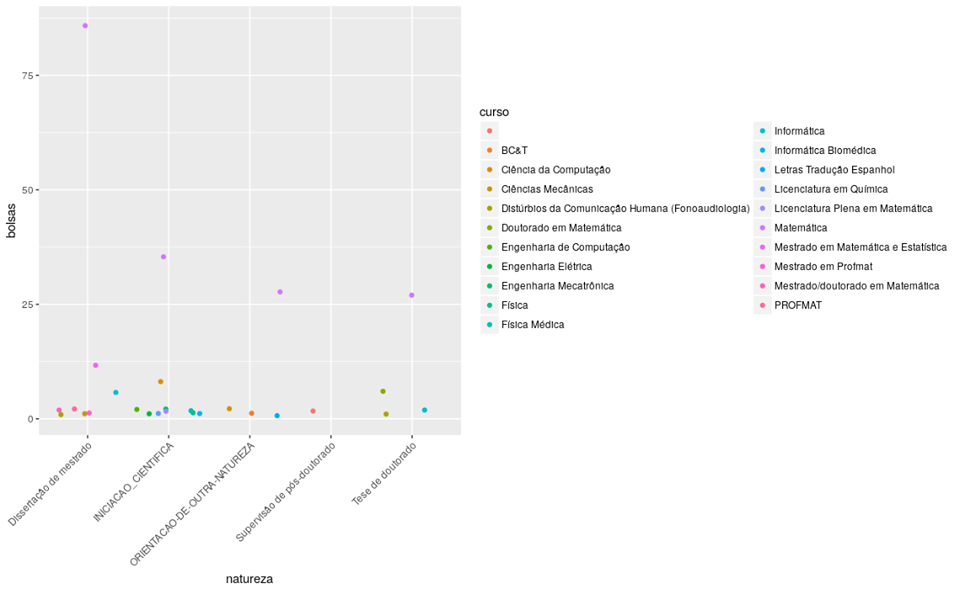
\includegraphics{graph.png}

Além disso, 2014 foi o ano com o maior número de bolsistas: 47 do total
de 236 bolsas avaliadas desde 2010. O número de bolsas sofreu um grande
aumento em relação à anos anteriores, o que indica crescimento e
desenvolvimento do programa desde 2010. Entretanto, em 2017 este número
caiu para 29. Que pode ser interpretado como uma reflexão do menor
número de mestrandos no programa ou um menor número de bolsas
disponíveis.

O ano de 2014 também foi o ano com resultados mais expressivos para
publicações do programa, conforme comentado anteriormente. Isso nos
mostra uma relação direta entre o número de bolsas para orientações e
publicações.

\begin{Shaded}
\begin{Highlighting}[]
\NormalTok{orientacoes <-}\StringTok{ }\KeywordTok{fromJSON}\NormalTok{(}\StringTok{"Matematica.advise.json"}\NormalTok{)}
\KeywordTok{names}\NormalTok{(orientacoes)}
\CommentTok{# orientacoes <- orientacoes[-4:-5] # Tirar dados da Graduação}
\KeywordTok{names}\NormalTok{(orientacoes)}

\KeywordTok{sum}\NormalTok{(}\KeywordTok{sapply}\NormalTok{(orientacoes}\OperatorTok{$}\NormalTok{ORIENTACAO_EM_ANDAMENTO_DE_POS_DOUTORADO, length))}
\KeywordTok{sum}\NormalTok{(}\KeywordTok{sapply}\NormalTok{(orientacoes}\OperatorTok{$}\NormalTok{ORIENTACAO_EM_ANDAMENTO_DOUTORADO, length))}
\KeywordTok{sum}\NormalTok{(}\KeywordTok{sapply}\NormalTok{(orientacoes}\OperatorTok{$}\NormalTok{ORIENTACAO_EM_ANDAMENTO_MESTRADO, length))}

\KeywordTok{sum}\NormalTok{(}\KeywordTok{sapply}\NormalTok{(orientacoes}\OperatorTok{$}\NormalTok{ORIENTACAO_CONCLUIDA_POS_DOUTORADO, length))}
\KeywordTok{sum}\NormalTok{(}\KeywordTok{sapply}\NormalTok{(orientacoes}\OperatorTok{$}\NormalTok{ORIENTACAO_CONCLUIDA_DOUTORADO, length))}
\KeywordTok{sum}\NormalTok{(}\KeywordTok{sapply}\NormalTok{(orientacoes}\OperatorTok{$}\NormalTok{ORIENTACAO_CONCLUIDA_MESTRADO, length))}

\NormalTok{ori.df <-}\StringTok{ }\KeywordTok{data.frame}\NormalTok{()}
\ControlFlowTok{for}\NormalTok{(i }\ControlFlowTok{in}\NormalTok{ orientacoes) \{}
  \ControlFlowTok{for}\NormalTok{(j }\ControlFlowTok{in}\NormalTok{ i) \{}
\NormalTok{    ori.df <-}\StringTok{ }\KeywordTok{rbind}\NormalTok{(ori.df, j)}
\NormalTok{  \}}
\NormalTok{\}}

\KeywordTok{glimpse}\NormalTok{(ori.df)}
\KeywordTok{unique}\NormalTok{(ori.df}\OperatorTok{$}\NormalTok{natureza)}
\KeywordTok{unique}\NormalTok{(ori.df}\OperatorTok{$}\NormalTok{curso)}

\NormalTok{ori.df}\OperatorTok{$}\NormalTok{curso <-}\StringTok{ }
\StringTok{  }\NormalTok{ori.df}\OperatorTok{$}\NormalTok{curso }\OperatorTok
\StringTok{    }\KeywordTok{str_replace_all}\NormalTok{(}\StringTok{"Dotorado em matemática"}\NormalTok{, }\StringTok{"Doutorado em Matemática"}\NormalTok{) }\OperatorTok
\StringTok{    }\KeywordTok{str_replace_all}\NormalTok{(}\StringTok{"Doutorado em Matematica"}\NormalTok{, }\StringTok{"Doutorado em Matemática"}\NormalTok{) }\OperatorTok
\StringTok{    }\KeywordTok{str_replace_all}\NormalTok{(}\StringTok{"Doutorado em matemática"}\NormalTok{, }\StringTok{"Doutorado em Matemática"}\NormalTok{) }\OperatorTok
\StringTok{    }\KeywordTok{str_replace_all}\NormalTok{(}\StringTok{"Matematica"}\NormalTok{, }\StringTok{"Matemática"}\NormalTok{) }\OperatorTok
\StringTok{    }\KeywordTok{str_replace_all}\NormalTok{(}\StringTok{"matemática"}\NormalTok{, }\StringTok{"Matemática"}\NormalTok{) }\OperatorTok
\StringTok{    }\KeywordTok{str_replace_all}\NormalTok{(}\StringTok{"matematica"}\NormalTok{, }\StringTok{"Matemática"}\NormalTok{) }\OperatorTok
\StringTok{    }\KeywordTok{str_replace_all}\NormalTok{(}\StringTok{"Ciências da Computação"}\NormalTok{, }\StringTok{"Ciência da Computação"}\NormalTok{)}

\NormalTok{ori.df }\OperatorTok
\StringTok{  }\KeywordTok{filter}\NormalTok{(bolsa }\OperatorTok{==}\StringTok{ "SIM"}\NormalTok{) }\OperatorTok
\StringTok{  }\KeywordTok{group_by}\NormalTok{(natureza, curso) }\OperatorTok
\StringTok{  }\KeywordTok{summarise}\NormalTok{(}\DataTypeTok{bolsas =} \KeywordTok{n}\NormalTok{()) }\OperatorTok
\StringTok{  }\KeywordTok{arrange}\NormalTok{(}\KeywordTok{desc}\NormalTok{(bolsas)) }\OperatorTok
\StringTok{  }\KeywordTok{ggplot}\NormalTok{(}\KeywordTok{aes}\NormalTok{(}\DataTypeTok{x =}\NormalTok{ natureza, }\DataTypeTok{y =}\NormalTok{ bolsas, }\DataTypeTok{col =}\NormalTok{ curso)) }\OperatorTok{+}
\StringTok{  }\KeywordTok{geom_jitter}\NormalTok{() }\OperatorTok{+}
\StringTok{  }\KeywordTok{theme}\NormalTok{(}\DataTypeTok{axis.text.x =} \KeywordTok{element_text}\NormalTok{(}\DataTypeTok{angle =} \DecValTok{45}\NormalTok{, }\DataTypeTok{hjust =} \DecValTok{1}\NormalTok{))}
\end{Highlighting}
\end{Shaded}

\includegraphics{Relatório_4_files/figure-latex/orientacoes-1.pdf}
\#\#AQUI VAI O DO PAULO

O dataset MatematicaRedeResearchers.json contém todas as áreas em que
existem algum tipo de produção científica, a nível de pós-graduação,
produzida ou em produção até 2017 por membros do Departamento de
Matemática. Como é possível notar os temas desenvolvidos não são
exculivamente da Matemática ou ainda das Ciências Exatas, existe uma
flexibilização que permite ao pesquisador trabalhar em diferentes campos
do saber. Outro dado interessante é o desenvolvimento de trabalhos na
área da educação o que valida as informações apresentadas no site do
departamento onde são apresentados diversos projetos nesse âmbito.

print(administração)

\#\# {[}1{]} 1

print(educação)

\#\# {[}1{]} 4

print(engBioMédica)

\#\# {[}1{]} 1

print(matemática)

\#\# {[}1{]} 26

print(ProbeEstat)

\#\# {[}1{]} 2

print(Psicologia)

\#\# {[}1{]} 2

Visando aprofundar as análises será dado foco ao grupo de quatro
pesquisadores do Departamento de Matemática que desenvolveram trabalhos
na área da Psicologia. Estes podem ser identifados pelo número de seu ID
do Currículo Lattes, como já é conhecido temos dois resultados:

\begin{verbatim}
##  chr [1:2] "0556476746202406" "5874654544324539"
\end{verbatim}

De posse dos IDs é possível fazer algumas observações, para tal foi
adicionado o dataset MatematicaRede.profile.json que contém o perfil
Lattes de todos os membros do departamento. De posse dessas informações
é possível comprovar a existência dos pesquisadores com os ID que foram
encontrados e ainda verificar se eles, mesmo sendo ``nativos'' da
Matemática, possuem alguma pesquisa na área da Psicologia olhando suas
áreas de atuação:

\begin{Shaded}
\begin{Highlighting}[]
\KeywordTok{str}\NormalTok{(pesq1 <-}\StringTok{ }\KeywordTok{data_frame}\NormalTok{(perfil}\OperatorTok{$}\StringTok{`}\DataTypeTok{0556476746202406}\StringTok{`}\OperatorTok{$}\NormalTok{areas_de_atuacao}\OperatorTok{$}\NormalTok{area))}
\end{Highlighting}
\end{Shaded}

\begin{verbatim}
## Classes 'tbl_df', 'tbl' and 'data.frame':    3 obs. of  1 variable:
##  $ perfil$`0556476746202406`$areas_de_atuacao$area: chr  "Matemática" "Educação" "Psicologia"
\end{verbatim}

\begin{Shaded}
\begin{Highlighting}[]
\KeywordTok{str}\NormalTok{(pesq2 <-}\StringTok{ }\KeywordTok{data_frame}\NormalTok{(perfil}\OperatorTok{$}\StringTok{`}\DataTypeTok{5874654544324539}\StringTok{`}\OperatorTok{$}\NormalTok{areas_de_atuacao}\OperatorTok{$}\NormalTok{area))}
\end{Highlighting}
\end{Shaded}

\begin{verbatim}
## Classes 'tbl_df', 'tbl' and 'data.frame':    4 obs. of  1 variable:
##  $ perfil$`5874654544324539`$areas_de_atuacao$area: chr  "Matemática" "Educação" "Educação" "Psicologia"
\end{verbatim}

Ainda sobre as áreas de pesquisa é possível notar, como talvez já fosse
esperado, que as sub-áreas da Matemáticas são majoritariamente as mais
buscadas para desenvolvimento de pesquisas e isso pode ser verificado no
gráfico a seguir que mostra a distribuição das pesquisas por área e
diante do número pode-se afirmar que as sub-áres da Matemática são as de
maior interesse e por consequência possuem os \textbf{resultados mais
relevantes}.
\includegraphics{Relatório_4_files/figure-latex/unnamed-chunk-18-1.pdf}

Limitando o escopo de análise aos pesquisadores que se dedicaram à
pesquisas envolvendo temas da Psicologia é interessante analisar que se
em algum momento antes de adquirirem seus títulos eles se dedicaram de
alguma forma ao estudo da Psicologia. Para isso é feita uma análise dos
resumos dos seus currículos Lattes. Devido

\begin{Shaded}
\begin{Highlighting}[]
\NormalTok{resumo_pesq1 <-}\StringTok{ }\NormalTok{(perfil}\OperatorTok{$}\StringTok{`}\DataTypeTok{0556476746202406}\StringTok{`}\OperatorTok{$}\NormalTok{resumo_cv )}
\NormalTok{resumo_pesq2 <-}\StringTok{ }\NormalTok{(perfil}\OperatorTok{$}\StringTok{`}\DataTypeTok{5874654544324539}\StringTok{`}\OperatorTok{$}\NormalTok{resumo_cv)}
\NormalTok{resumo_pesq1}
\end{Highlighting}
\end{Shaded}

\begin{verbatim}
## [1] "Professor Associado I na Universidade de Brasília - UnB, com lotação no Departamento de Matemática. É membro do Programa de Pós-Graduação em Educação da UnB, orientando pesquisas nos cursos de mestrado acadêmico e doutorado em educação. Possui graduação em Licenciatura em Ciências e Matemática pelo Centro Universitário de Brasília (1991), mestrado em Educação pela Universidade de Brasília (1999) e doutorado em Psicologia pela Universidade de Brasília (2007). Tem experiência na área de Matemática, com ênfase em Educação Matemática, atuando principalmente nos seguintes temas: criatividade em matemática, avaliação em matemática e resolução de problemas."
\end{verbatim}

\begin{Shaded}
\begin{Highlighting}[]
\NormalTok{resumo_pesq2}
\end{Highlighting}
\end{Shaded}

\begin{verbatim}
## [1] "Possui Licenciatura em Matemática (1995) e Especialização em Matemática (1998) pela Universidade Federal de Goiás, Mestrado em Educação (2002) e Doutorado em Psicologia (2008) pela Universidade de Brasília. Tem experiência profissional: 1) na Educação Básica como docente de matemática e coordenadora de área em instituições de ensino públicas e particulares; 2) no Ensino Superior como docente nos Cursos de Licenciatura em Matemática e Pedagogia e Coordenadora do Curso de Licenciatura em Matemática; 3) na pós-graduação como docente dos cursos de Especialização em Educação Matemática e Psicopedagogia;coordenadora do Curso de Especialização em Educação Matemática; 4) na Educação à Distância como tutora, formadora e autora de material didático para a formação continuada de professores que ensinam matemática (Ensino Fundamental Anos Iniciais e Finais; Ensino Médio) e alfabetizadores de Jovens e Adultos; Atuou como primeira secretária da Sociedade Brasileira de Educação Matemática (gestão 2010-2013); Desenvolve consultorias desde 2002 para o Ministério da Educação (MEC), Instituto Nacional de Estudos e Pesquisas Educacionais Anísio Teixeira (Inep) e Secretarias Estaduais de Educação nas áreas de tecnologia educacional, formação de professores (presencial, semipresencial e à distância) e avaliação em matemática; Atualmente é professora adjunta, coordenadora da comissão de extensão e membro do Núcleo Docente Estruturante (NDE) do Departamento de Matemática da Universidade de Brasília(UnB); Coordenadora da Extensão do Instituto de Exatas; Docente do Programa de Pós-Graduação do Instituto de Exatas, Mestrado Profissional em Matemática (PROFMat/IE/UnB); Colaboradora do Programa de Pós-graduação em Educação da Faculdade de Educação (UnB); Colaboradora do Curso de Especialização em Psicopedagogia Clínica e Institucional, do Instituto de Psicologia (UnB); Diretora da Sociedade Brasileira de Educação Matemática - Regional Distrito Federal; Membro dos seguintes Grupos de Pesquisa: Grupo de Investigação em Educação Matemática da UnB; Grupo de Pesquisas Interdisciplinares sobre Tecnologias e Educação (ÁBACO/FE/UnB); Grupo de Pesquisas e Investigações em Educação Matemática (PI/FE/UnB) e Grupo de pesquisa em Psicologia do Conhecimento (COGITO). Coordenadora Geral da I Feira de Matemática do Distrito Federal, realizada no dia 01.09.2017 e do VII Encontro Brasiliense de Educação Matemática, realizado nos dias 01,02 e 03.09.2017."
\end{verbatim}

Outro dado interessante é analisar o nível de internacionalização das
produções dos pesquisadores, isso pode ser analisado com a quantidade de
participações em eventos internacionais e nacionais.Como é possível ver
através dos gráficos a internacionalização das pequisas pode ser
considerada baixa, porém existe forte participação desses pesquisadoes
em âmbito nacional.

\paragraph{Pesquisador
ID\_0556476746202406}\label{pesquisador-id_0556476746202406}

\includegraphics{Relatório_4_files/figure-latex/unnamed-chunk-20-1.pdf}

\paragraph{Pesquisador
ID\_5874654544324539}\label{pesquisador-id_5874654544324539}

\includegraphics{Relatório_4_files/figure-latex/unnamed-chunk-21-1.pdf}

\section{CRISP-DM Fase.Atividade 5 - conclusões dos relatorios
3}\label{crisp-dm-fase.atividade-5---conclusoes-dos-relatorios-3}

\subsection{Quanto ao PPG de ensino de
ciências}\label{quanto-ao-ppg-de-ensino-de-ciencias}

Portanto podemos observar que o programa de pós-graduação de ensino em
ciências apresenta um baixo nível de internacionalização uma vez que
grande parte de suas produções e orientações são voltadas a alunos de
instituições nacionais e a periódicos nacionais em sua grande maioria
publicados em língua portuguesa do Brasil.

É importante também notar que o programa possui um grande grau de
colaboração entre seus participantes uma vez que a maior parte das
publicações são realizadas em grupos, assim como as produções literárias
e artigos produzidos. Também foram observadas mudanças nas produções do
departamento ao longo dos últimos anos que podem ser analisadas mais a
fundo, aqui foi proposta uma relação com cortes de fundos mas que devem
ser avaliados traçando relações com informações sobre o cenário
brasileiro.

Algumas informações sobre a mudança no quadro de funcionários também foi
levantada durante a pesquisa e poderá também ser avaliada com mais
profundidade para averiguar qual o real impacto disso no programa.

\subsection{AQUI VAI O DO PAULO}\label{aqui-vai-o-do-paulo}

O simples estudo dos datasets da Matemática permitiu tirar conclusões
acerca de seu programa de pós-graduação e validar as informações
contidas no site do programa. Assim como havia sido afirmado
anteriormente o Departamento é capaz de oferecer oportunidades de estudo
em diversos campos do saber, ainda assim não deixa de privilegiar as
sub-áreas das Ciências Exatas como a Álgebra e a Estatística. De acordo
com os resultados obtidos é possível notar que as áreas de pós-graduação
dentro da Matemática que não trabalham diretamente com sub-áreas das
exatas não possuem o mesmo grau de internacionalização que as demais,
porém por serem numericamente inferiores não tem impacto direto na nota
do curso que é alta, outra informação que foi validade de acordo com o
que está no site do programa.

\section{CRISP-DM Fase.Atividade 6}\label{crisp-dm-fase.atividade-6}

De que forma os produtos desenvolvidos pelo grupo poderiam ser colocados
em uso prático regular, na organização cliente?

\subsection{CRISP-DM Fase.Atividade 6.2 - Planejamento do monitoramento
dos
produtos}\label{crisp-dm-fase.atividade-6.2---planejamento-do-monitoramento-dos-produtos}

De que forma seria possível realizar o monitoramento do funcionamento
dos produtos em utilização no ambiente operacional?

\subsection{CRISP-DM Fase.Atividade 6.3 - Planejamento de
manuteção}\label{crisp-dm-fase.atividade-6.3---planejamento-de-manutecao}

que manutenções, ajustes, mudanças, poderia ter que ser eventualmente
realizadas no produto (scripts), quando em uso no ambiente operacional
do cliente?

\subsection{CRISP-DM Fase.Atividade 6.6 - Revisão sobre a execução do
projeto}\label{crisp-dm-fase.atividade-6.6---revisao-sobre-a-execucao-do-projeto}

O trabalho feito visou o estudo de tudo aquilo que é produzido
cientificamente pela universidade (ciência da ciência) e qual a
relevância destas descobertas para os próprios pesquisadores e alunos,
com o intuito de validarem o método que utilizam e a qualidade daquilo
que vem sendo criado.

A mais antiga das ciências da ciência é a filosofia. A tarefa da
filosofia consistiu, durante séculos, em estabelecer o melhor método do
conhecimento verdadeiro, e depois aplicá-lo para o entendimento do
mundo, da religião e da moral. A ciência da ciência é hoje uma atividade
multi-disciplinar, com muitas abordagens distintas.

O pensamento lógico já se demonstrou ineficiente para criação de teorias
científicas e para descrever a natureza. René Descartes, já afirmava
que: ``Matemática é uma ferramenta para se fazer ciência, mas não é uma
ciência''. Isso ocorre, pois palavras e números não existem na natureza,
portanto não são ciência. Mas, a matemática já se mostrou ótima
ferramenta para o estudo e formulação de teorias científicas.

A Matemática é essencial para muitas ciências. A função mais importante
da Matemática na ciência é o papel que ela possui na expressão de
modelos científicos. Medidas de coleta e observação, bem como
hipotetizar e prever, geralmente requerem modelos matemáticos e um
extensivo uso da Matemática. Os ramos matemáticos mais utilizados na
ciência incluem o cálculo e a estatística, apesar de virtualmente cada
ramo da Matemática ter aplicações, mesmo áreas ``puras'' tais como a
teoria numérica e a topologia. A Matemática prevalece mais na Física, e
menos em Química e algumas ciências sociais. Alguns pensadores vêem os
matemáticos como cientistas, considerando os experimentos físicos como
não essenciais ou as provas matemáticas como equivalentes a
experimentos. Outros não vêem a Matemática como ciência, já que ela não
requer teste experimental de suas teorias e hipóteses. Em qualquer caso,
o fato de que a Matemática é uma ferramenta útil na descrição do
universo é uma questão da Filosofia da Matemática. Richard Feynman
disse: ``A Matemática não é real, mas se sente real. Onde é esse
lugar?'', enquanto que a definição favorita de Bertrand Russell sobre a
Matemática é ``o assunto no qual nunca sabemos do que estamos falando
nem se o que estamos dizendo está certo.''

O programa de pós-graduação sendo avaliado gerou ao longo dos anos
diversos subprodutos que são consequências direta da atividade
cientifica como por exemplo publicações e ou orientações acadêmicas que
podem ser avaliadas para gerar um feedback qualitativo sobre o programa.
Algumas questões devem ser levantadas ao realizar estes estudos, entre
elas como definir uma métrica para o que está sendo avaliado? Sabemos
que grande parte das bases de dados internacionais indexam apenas
pesquisas realizadas em língua inglesa, portanto como é possível avaliar
o impacto internacional do que é produzido no país?

Estas questões são discutidas e exploradas na ciência da ciência poís
devemos ser capazes de medir e validar o impacto do que é produzido em
nossas universidade e como é possível melhorar o que vem sendo
produzido. Existem grupos de pesquisa como por exemplo o Science and
Evaluation Studies(SES) que se dedicam exclusivamente ao estudo de
métricas de avaliações de pesquisas cientificas.

A plataforma Lattes vem com o objetivo de auxiliar nos estudos acerca da
produção realizada na universidade. Diversos conjuntos de dados
acadêmicos são agregados com o intuito de gerar um material organizado e
padronizado para que outros usuários possam disfrutar destas
informações. Os estudos aqui realizados se baseiam nos conjuntos de
dados fornecidos a respeito de publicações, orientações e perfis
agregados pela própria plataforma do Lattes que se tornou bastante
relevante no momento de definir nossas métricas de avaliação.

\section{Referências}\label{referencias}

\begin{itemize}
\tightlist
\item
  Azevedo, Mário Luiz Neves de, João Ferreira de Oliveira, e Afrânio
  Mendes Catani. ``O Sistema Nacional de Pós-Graduação (SNPG) e o Plano
  Nacional de Educação (PNE 2014-2024): regulação, avaliação e
  financiamento''. Revista Brasileira de Política e Administração da
  Educação 32, nº 3 (2016).
  \url{http://dx.doi.org/10.21573/vol32n32016.68576}.
\item
  Can, Fazli, Tansel Özyer, e Faruk Polat, orgs. State of the Art
  Applications of Social Network Analysis. Lecture Notes in Social
  Networks. Switzerland: Springer International Publishing, 2014.
\item
  CAPES. ``Documentos de Área''. CAPES.gov.br. Acessado 12 de junho de
  2018.
  \url{http://avaliacaoquadrienal.capes.gov.br/documentos-de-area}.
\item
  ---------. ``Plano Nacional de Pós-Graduação - PNPG 2011/2020 Vol.
  1''. Brasília - DF, dezembro de 2010.
  \url{http://www.capes.gov.br/images/stories/download/Livros-PNPG-Volume-I-Mont.pdf}.
\item
  ---------. ``Plano Nacional de Pós-Graduação - PNPG 2011/2020 Vol.
  2''. Brasília - DF, dezembro de 2010.
  \url{http://www.capes.gov.br/images/stories/download/PNPG_Miolo_V2.pdf}.
\item
  ---------. ``Sucupira: coleta de dados, docentes de pós-graduação
  stricto sensu no Brasil 2015''. CAPES - Banco de Metadados, 16 de
  março de 2016.
  \url{http://metadados.capes.gov.br/index.php/catalog/63}.
\item
  Chapman, Pete, Julian Clinton, Randy Kerber, Thomas Khabaza, Thomas
  Reinartz, Colin Shearer, e Rüdiger Wirth. ``CRISP-DM 1.0: Step-by-Step
  Data Mining Guide''. USA: CRISP-DM Consortium, 2000.
  \url{https://www.the-modeling-agency.com/crisp-dm.pdf}.
\item
  Datacamp. ``Machine Learning with R (Skill Track)''. Datacamp, 2018.
  \url{https://www.datacamp.com/tracks/machine-learning}.
\item
  Fernandes, Jorge H C, e Ricardo Barros Sampaio. ``DataScienceForAll''.
  Zotero, 13 de junho de 2018.
  \url{https://www.zotero.org/groups/2197167/datascienceforall}.
\item
  ---------. ``Especificação do Trabalho Final da Disciplina de Ciência
  de Dados para Todos 2017.2: Estudo sobre a visibilidade internacional
  da produção científica das pós-graduações vinculadas às áreas de
  conhecimento da CAPES, na Universidade de Brasília (Comunicação
  Interna)''. Disciplina 116297 - Tópicos Avançados em Computadores,
  turma D, do semestre 2017.2, do Departamento de Ciência da Computação
  do Instituto de Ciências Exatas da Universidade de Brasília, 28 de
  novembro de 2017.
  \url{https://aprender.ead.unb.br/pluginfile.php/474549/mod_resource/content/1/Estudo\%20da\%20Cie\%CC\%82ncia.pdf}.
\item
  Fernandes, Jorge H C, Ricardo Barros Sampaio, e João Ribas de Moura.
  ``Ciência de Dados para Todos (Data Science For All) - 2018.1 -
  Análise da Produção Científica e Acadêmica da Universidade de Brasília
  - Modelo de Relatório Final da Disciplina - Departamento de Ciência da
  Computação da UnB''. Disciplina 116297 - Tópicos Avançados em
  Computadores, turma D, do semestre 2018.1, do Departamento de Ciência
  da Computação do Instituto de Ciências Exatas da Universidade de
  Brasília, 13 de junho de 2018.
\item
  Frickel, Scott, e Kelly Moore. The New Political Sociology of Science:
  Institutions, Networks, and Power. Science and technology in society.
  USA: The University of Wisconsin Press, 2006.
\item
  Graduate Prospects Ltd. ``Job profile: Higher education lecturer'',
  2018.
  \url{https://www.prospects.ac.uk/job-profiles/higher-education-lecturer}.
\item
  Kalpazidou Schmidt, Evanthia, e Ebbe Krogh Graversen. ``Persistent
  factors facilitating excellence in research environments''. Higher
  Education 75, nº 2 (1º de fevereiro de 2018): 341--63.
  \url{https://doi.org/10.1007/s10734-017-0142-0}.
\item
  Kilduff, Martin, e Wenpin Tsai. Social Networks and Organizations. UK:
  Sage Publications, 2003.
\item
  Kolaczyk, Eric D., e Gábor Csárdi. Statistical Analysis of Network
  Data with R. USA: Springer, 2014.
\item
  Kuhn, Max, Jed Wing, Steve Weston, Andre Williams, Chris Keefer, Allan
  Engelhardt, Tony Cooper, et al. ``Package `Caret' - Classification and
  Regression Training'', 27 de maio de 2018.
  \url{https://cran.r-project.org/web/packages/caret/caret.pdf}.
\item
  Leite, Fernando César Lima. ``Considerações básicas sobre a Avaliação
  do Sistema Nacional de Pós-Graduação''. Comunicação Pessoal (slides).
  Universidade de Brasília, abril de 2018.
  \url{https://aprender.ead.unb.br/pluginfile.php/502250/mod_resource/content/1/Considera\%C3\%A7\%C3\%B5es\%20b\%C3\%A1sicas\%20sobre\%20a\%20Avalia\%C3\%A7\%C3\%A3o\%20do\%20Sistema\%20Nacional.pdf}.
\item
  Lusher, Dean, Johan Koskinen, e Garry Robins, orgs. Exponential Random
  Graph Models for Social Networks: Theory, methods, and applications.
  Structural Analysis in the Social Sciences. USA: Cambridge University
  Press, 2013.
\item
  Mariscal, Gonzalo, Óscar Marbán, e Covadonga Fernández. ``A survey of
  data mining and knowledge discovery process models and
  methodologies''. The Knowledge Engineering Review 25, nº 2 (2010):
  137--66. \url{https://doi.org/10.1017/S0269888910000032}.
\item
  Nery, Guilherme, Ana Paula Bragaglia, Flávia Clemente, e Suzana
  Barbosa. ``Nem tudo parece o que é: Entenda o que é plágio''.
  Instituto de Arte e Comunicação Social da UFF, 2009.
  \url{http://www.noticias.uff.br/arquivos/cartilha-sobre-plagio-academico.pdf}.
\item
  Nooy, Wouter de, Andrej Mrvar, e Vladimir Batagelj. Exploratory Social
  Network Analysis with Pajek. Structural Analysis in the Social
  Sciences. USA: Routldge, 2005.
\item
  Pátaro, Cristina Saitê de Oliveira, e Frank Antonio Mezzomo. ``Sistema
  Nacional de Pós-Graduação no Brasil: estrutura, resultados e desafios
  para política de Estado - Lívio Amaral''. Revista Educação e
  Linguagens 2, nº 3 (julho de 2013): 11--17.
\item
  Schwartzman, Simon. ``A Ciência da Ciência''. Ciência Hoje 2, nº 11
  (março de 1984): 54--59.
\item
  Silver, Nate. The Signal and the Noise: Why so many predictions fail
  --- but some don't. USA: The Penguin Press HC, 2012.
\item
  Vicari, Donatella, Akinori Okada, Giancarlo Ragozini, e Claus Wiehs.
  Analysis and Modeling of Complex Data in Behavioral and Social
  Sciences. Studies in Classifi cation, Data Analysis, and Knowledge
  Organization. Switzerland: Springer, 2014.
\item
  Wickham, Hadley, e Garrett Grolemund. R for Data Science: Import,
  Tidy, Transform, Visualize, and Model Data. USA: O'Reilly, 2016.
\end{itemize}


\end{document}
